\chapter{Analisis}
\label{chap:analisis}

Pada bab ini akan dijelaskan mengenai analisis aplikasi sejenis yang menggunakan \textit{smartphone} sebagai pengendali permainan berbasis web, analisis \textit{sequence} diagram.

\section{Analisis Aplikasi Sejenis}
\label{sec:AirConsole}

Salah satu aplikasi sejenis permainan berbasis web dengan memanfaatkan \textit{smartphone} sebagai pengendali yaitu AirConsole. Aplikasi tersebut memanfaatkan teknologi \textit{browser}, \textit{smartphone}, \textit{PC}, dan juga jaringan internet untuk dapat menggunakannya. Aplikasi ini dikembangkan oleh N-Dream AG.

\textbf{Analisis AirConsole} 

AirConsole merupakan permainan berbasis web dimana \textit{browser} pada \textit{mobile device} dapat melakukan koneksi ke \textit{browser} pada  \textit{PC}. Pada aplikasi ini, terdapat berbagai macam permainan yang dapat dipilih oleh pemain. Untuk dapat memainkan aplikasi tersebut, pemain harus membuka alamat web \textit{airconsole.com} pada \textit{PC browser} dan juga pada \textit{smartphone browser}.

Analisis dilakukan dengan cara berikut:
\begin{enumerate}
	\item Memainkan permainan dari awal hingga akhir.
	\item Keluar dari \textit{browser} pada \textit{PC} pada saat permainan berlangsung.
	\item Keluar dari \textit{browser} pada \textit{smartphone} pada saat permainan berlangsung.
\end{enumerate}
Pada halaman awal web di \textit{PC}, pemain diminta untuk menekan tombol \textit{start} yang ada pada gambar berikut: 

\begin{figure}[H]
	\centering
	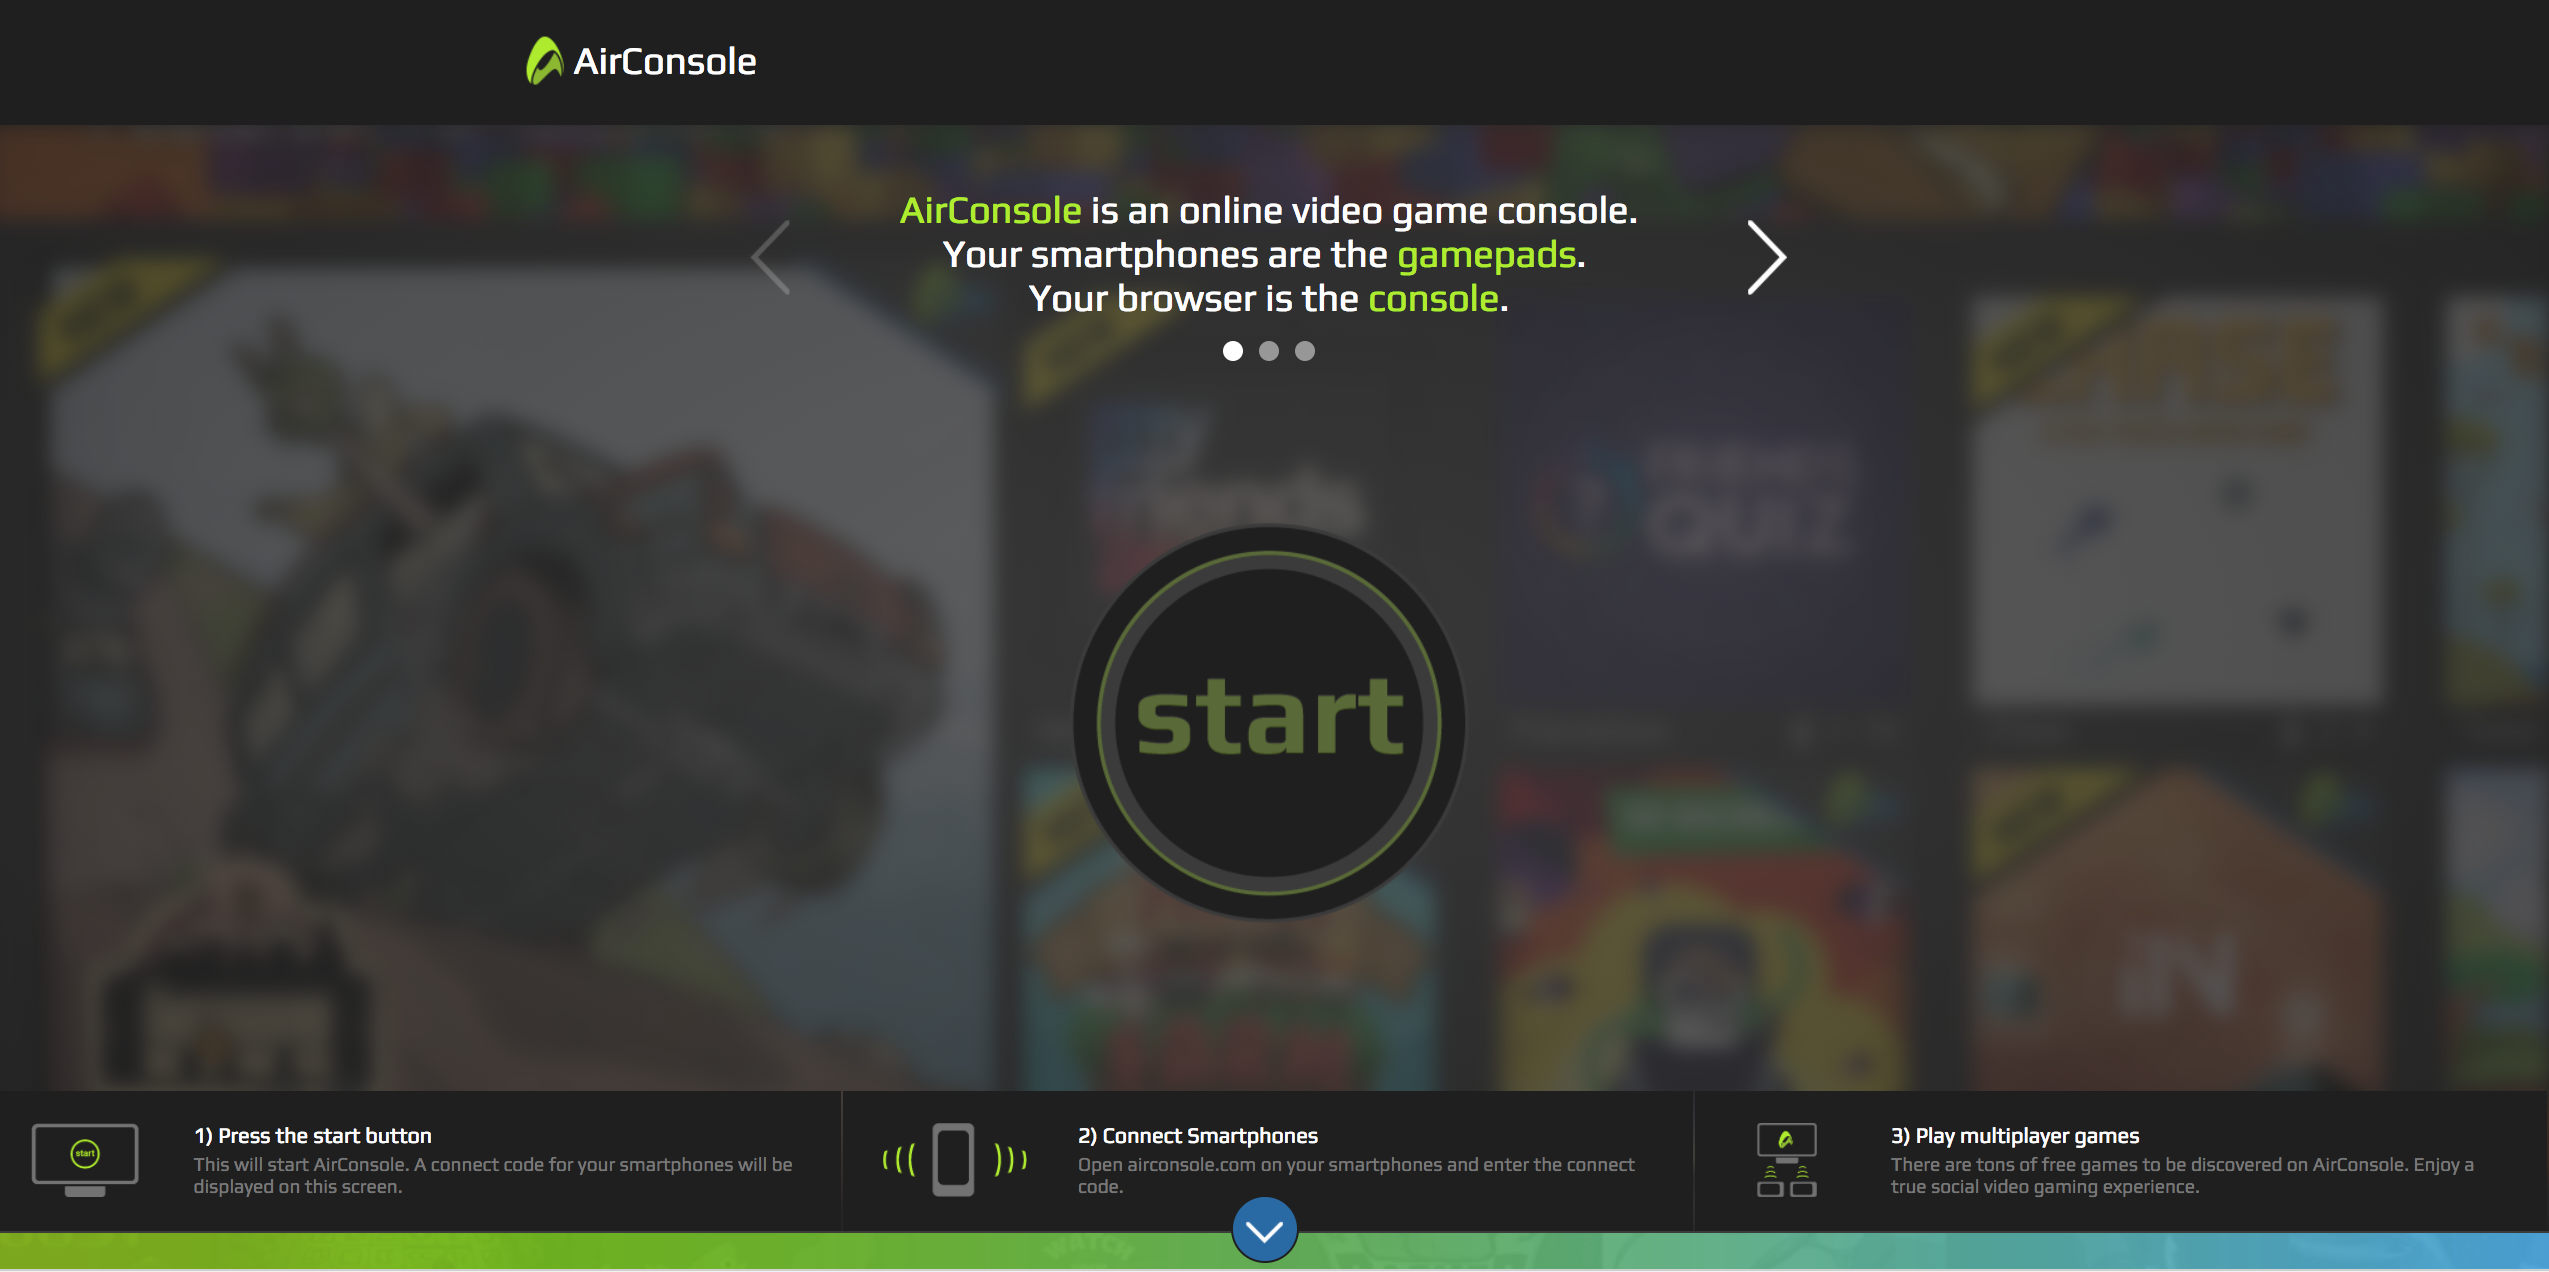
\includegraphics[scale=0.3]{Gambar/con1_home1}
	\caption{Halaman awal web pada \textit{PC browser}.}
	\label{fig:16_con1_home1}
\end{figure}

Setelah tombol \textit{start} ditekan, maka akan muncul halaman berikutnya yang menunjukan kode yang harus dimasukan oleh pemain pada \textit{mobile browser}. 

\begin{figure}[H]
	\centering
	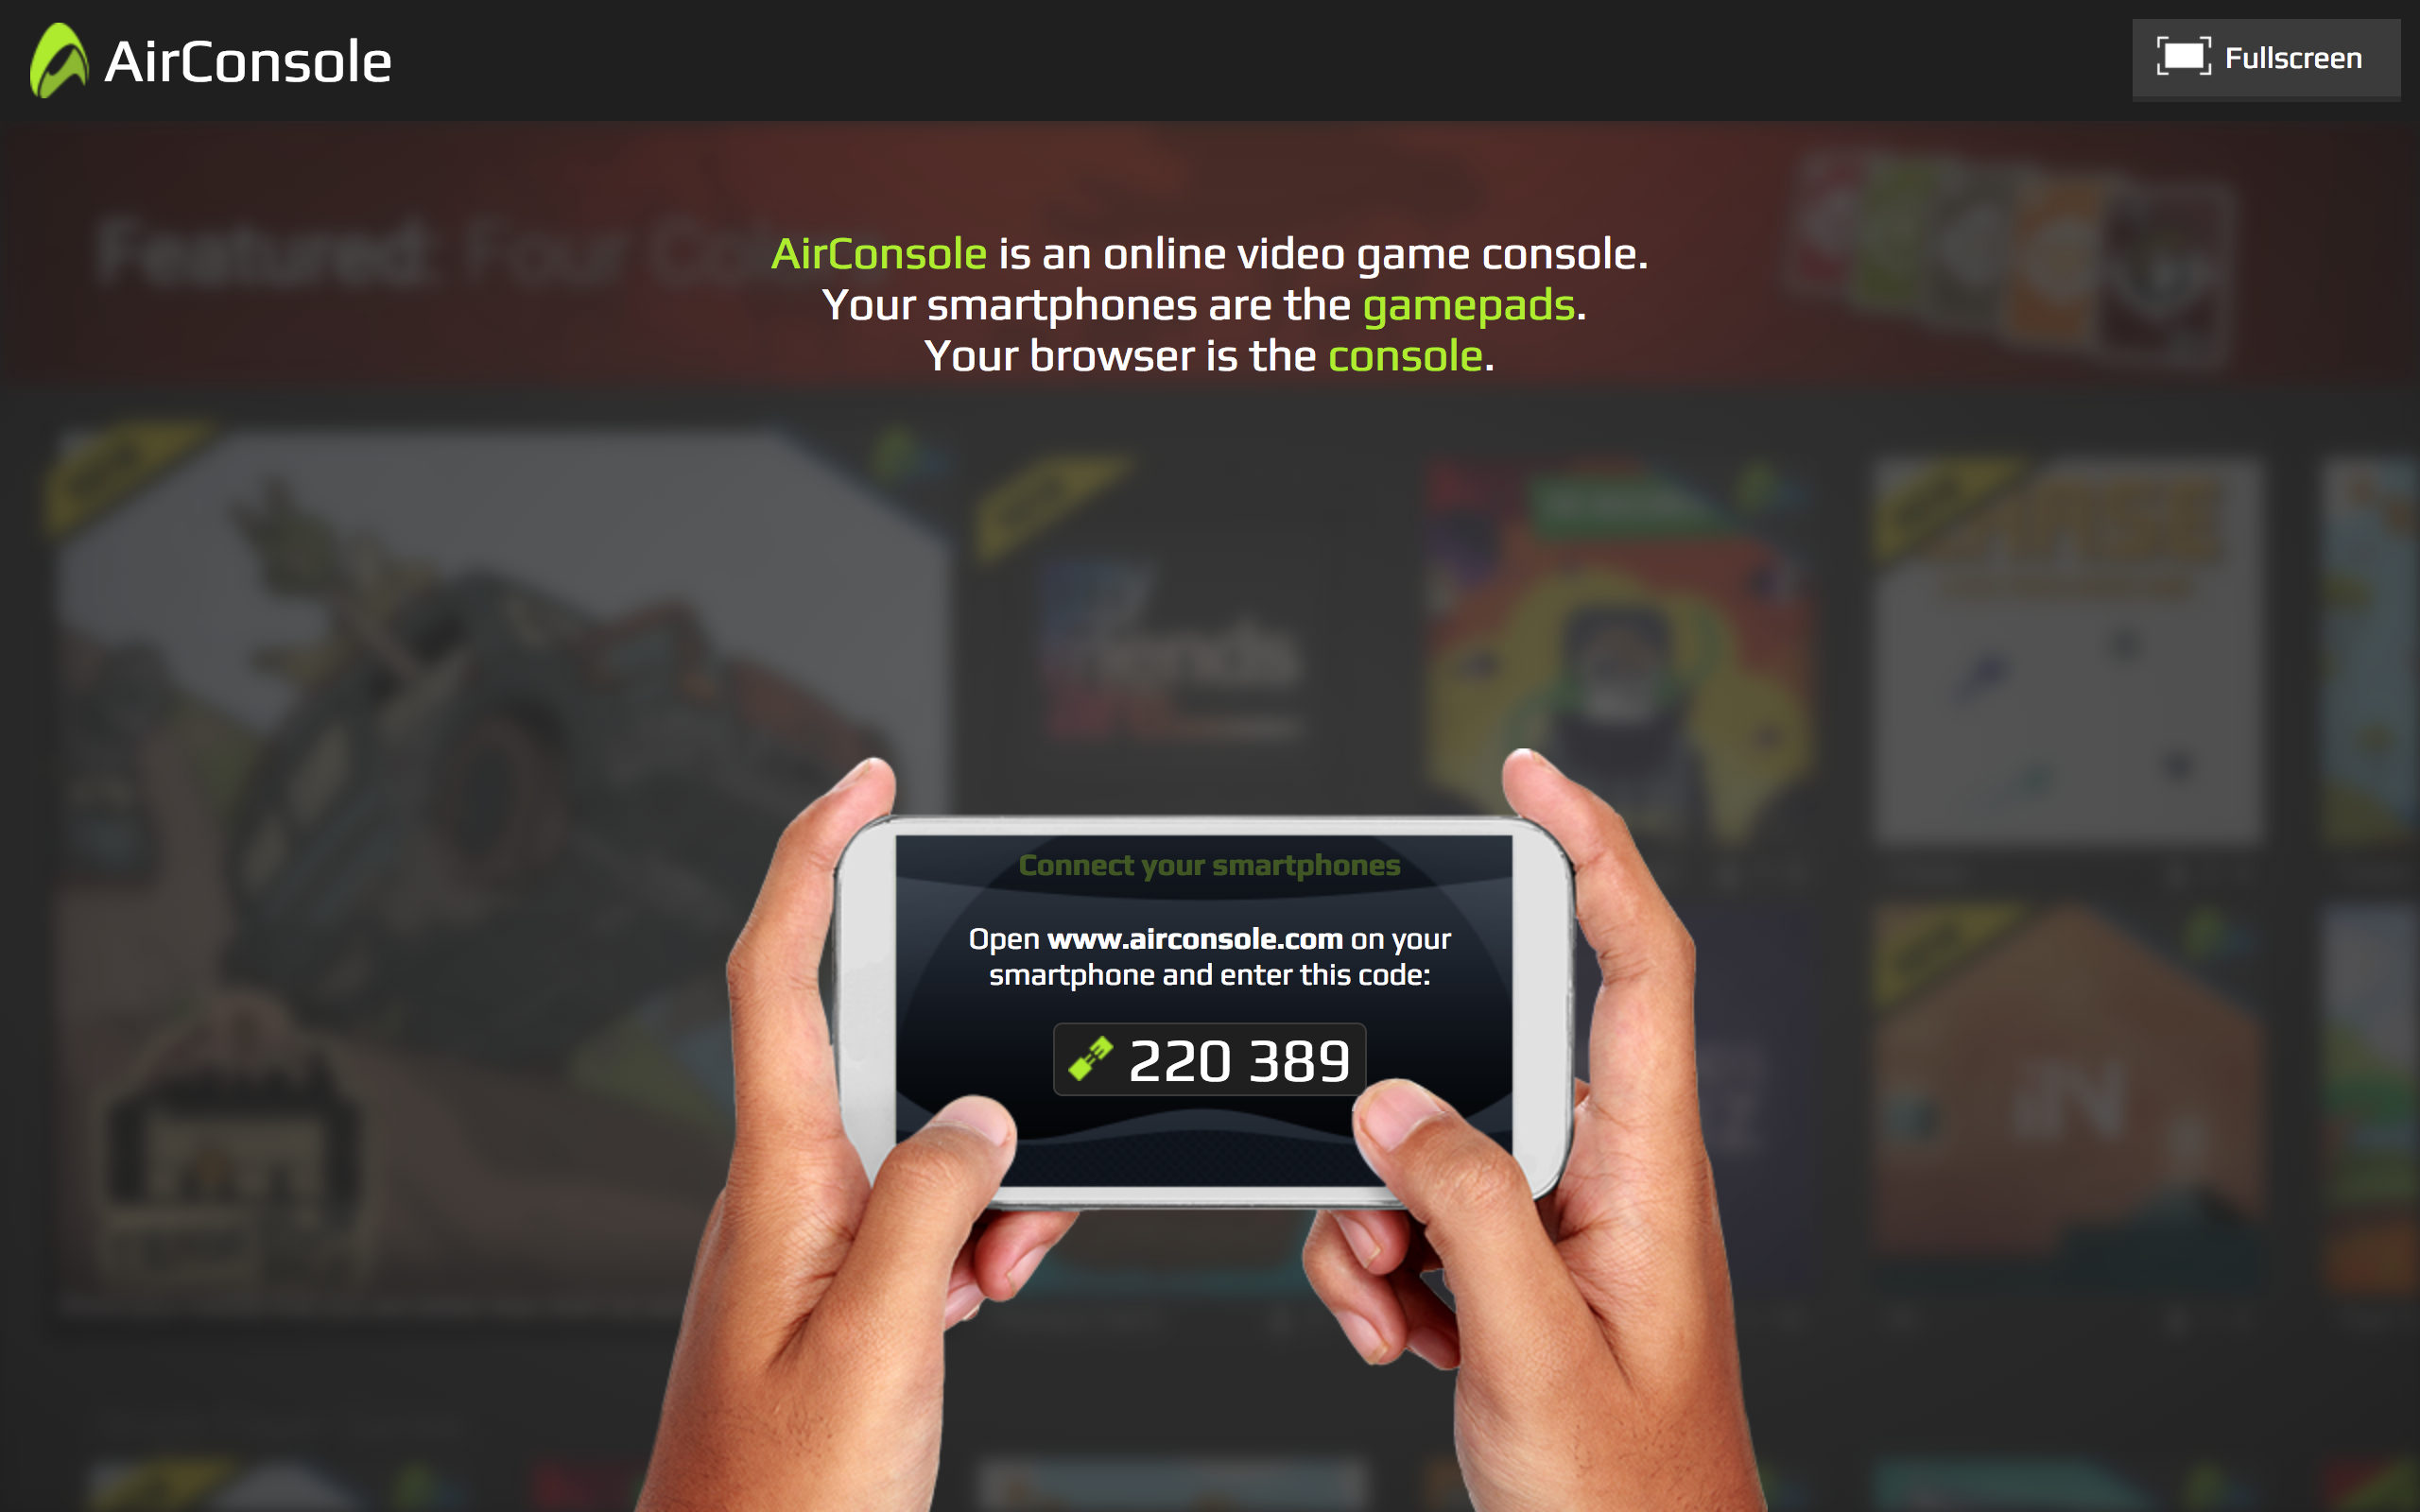
\includegraphics[scale=0.3]{Gambar/con2_code1}
	\caption{Kode yang harus dimasukan oleh pemain pada \textit{mobile browser}.}
	\label{fig:17_con2_code1}
\end{figure}

Pemain harus mengakses alamat web yang sama pada \textit{mobile browser}. Pada halaman awal, pemain akan diminta untuk memilih apakah akan bermain dengan menggunakan aplikasi, atau bermain dengan menggunakan \textit{browser}. 

\begin{figure}[H]
	\centering
	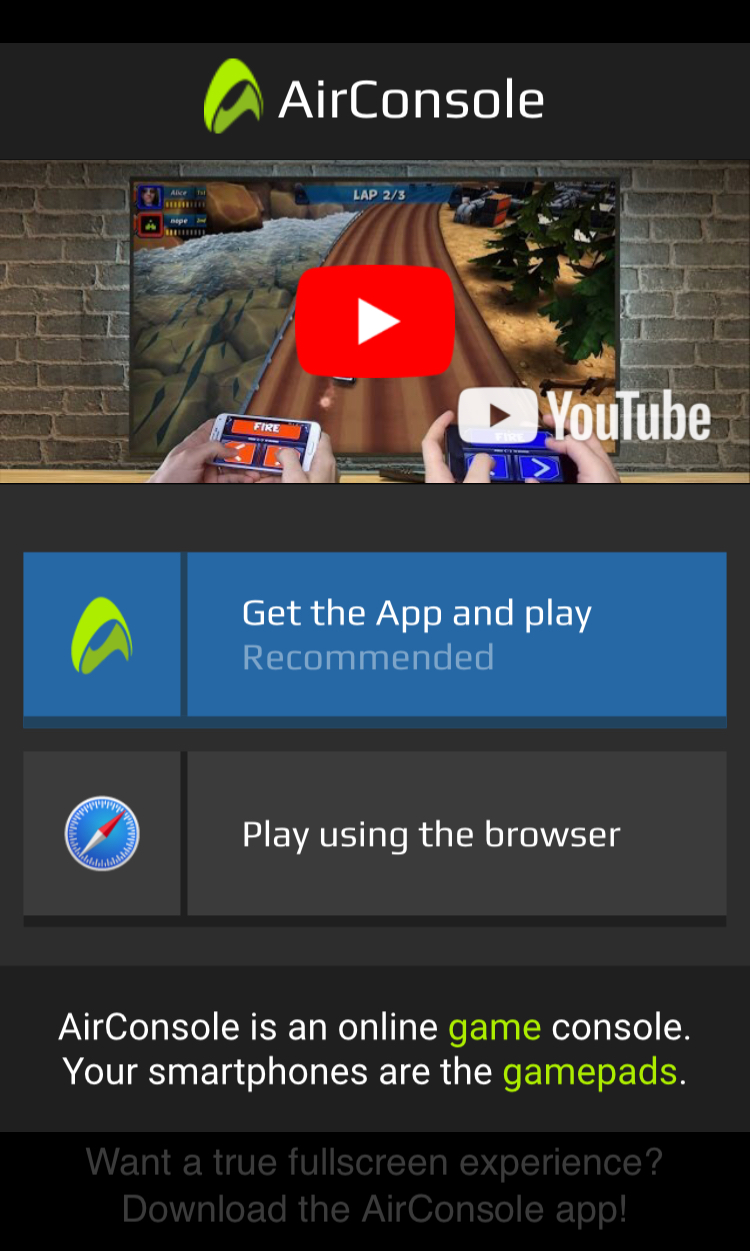
\includegraphics[scale=0.3]{Gambar/air1_home}
	\caption{Halaman awal pada \textit{mobile browser}.}
	\label{fig:18_air1_home}
\end{figure}

\vspace{-3cm}

Dalam analisis ini, penulis memilih untuk bermain menggunakan \textit{browser}. Setelah itu, pemain diminta untuk menekan tombol \textit{'i got the connect code'} untuk memasukan kode yang sudah didapatkan pada \textit{PC browser}.

\begin{figure}[H]
	\centering
	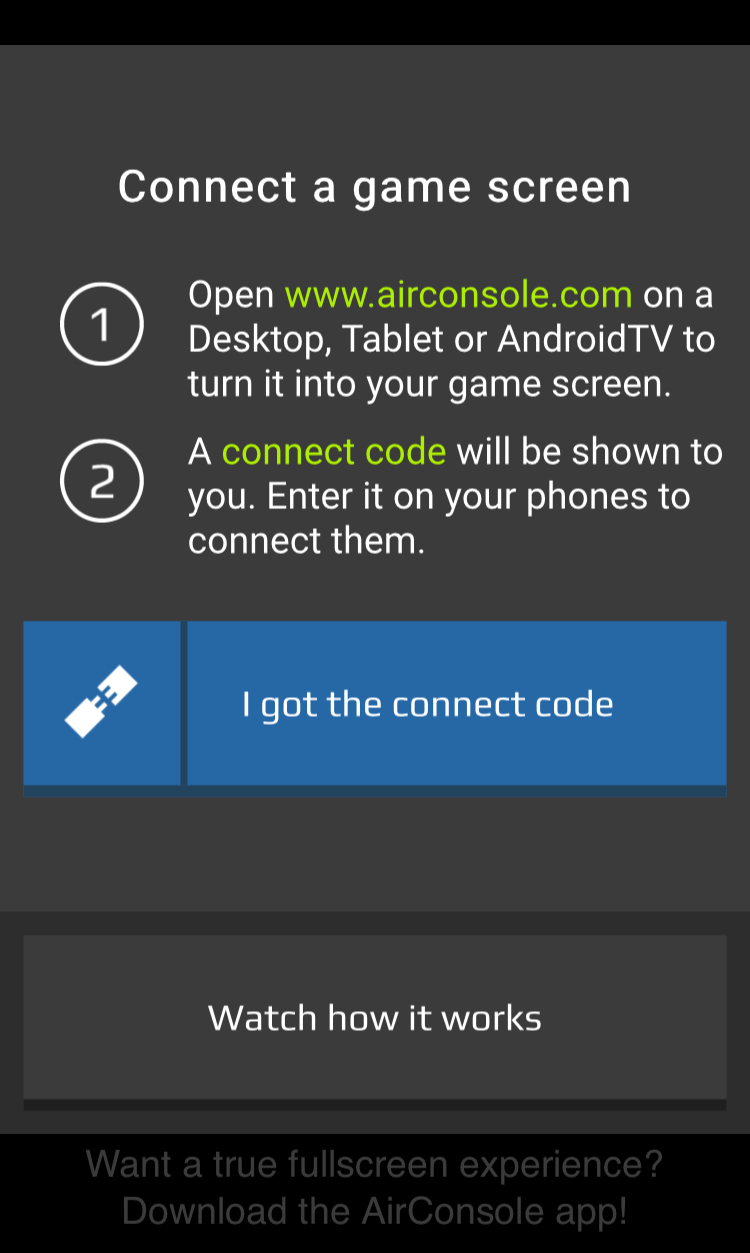
\includegraphics[scale=0.3]{Gambar/air2_code1}
	\caption{Pemain diminta untuk memasukan kode yang sudah didapatkan pada \textit{PC browser}.}
	\label{fig:19_air2_code1}
\end{figure}


Setelah menekan tombol tersebut, pemain dapat mulai memasukan kode yang sudah didapatkan. Kode ini bertujuan untuk proses otentikasi, sehingga para pemain yang dapat bermain dalam satu sesi yang sama, hanya para pemain yang mengetahui kode tersebut.

\begin{figure}[H]
	
	\centering
	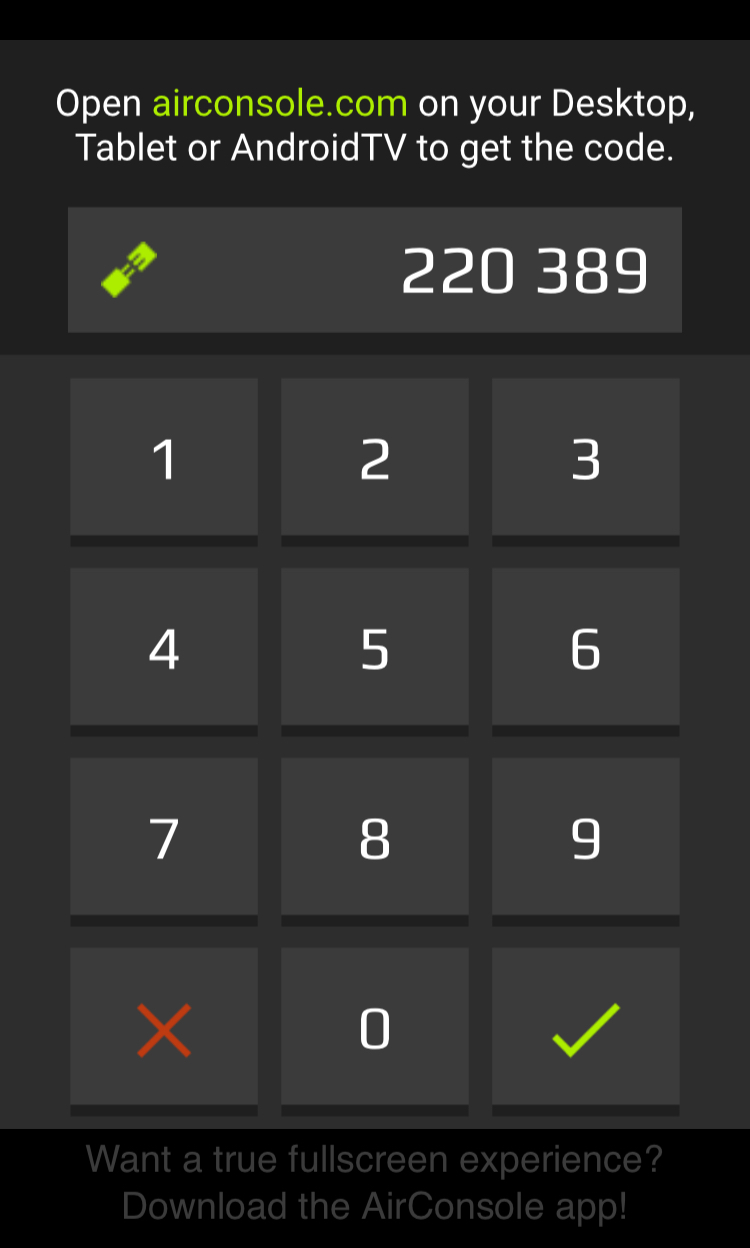
\includegraphics[scale=0.3]{Gambar/air3_code2}
	\caption{Pemain diminta untuk memasukan kode yang sudah didapatkan pada \textit{PC browser}.}
	\label{fig:20_air3_code2}
	
	
\end{figure}


Setelah pemain memasukan kode, maka halaman web di \textit{PC} dan \textit{smartphone} akan berubah. Pada \textit{PC}, halaman akan menunjukan berbagai jenis permainan yang dapat dipilih. Pada \textit{smartphone}, halaman akan berubah menjadi pengendali permainan, dimana pemain dapat menggerakan halaman yang ada di \textit{PC} dengan menggunakan \textit{smartphone}.

\begin{figure}[H]
	\centering
	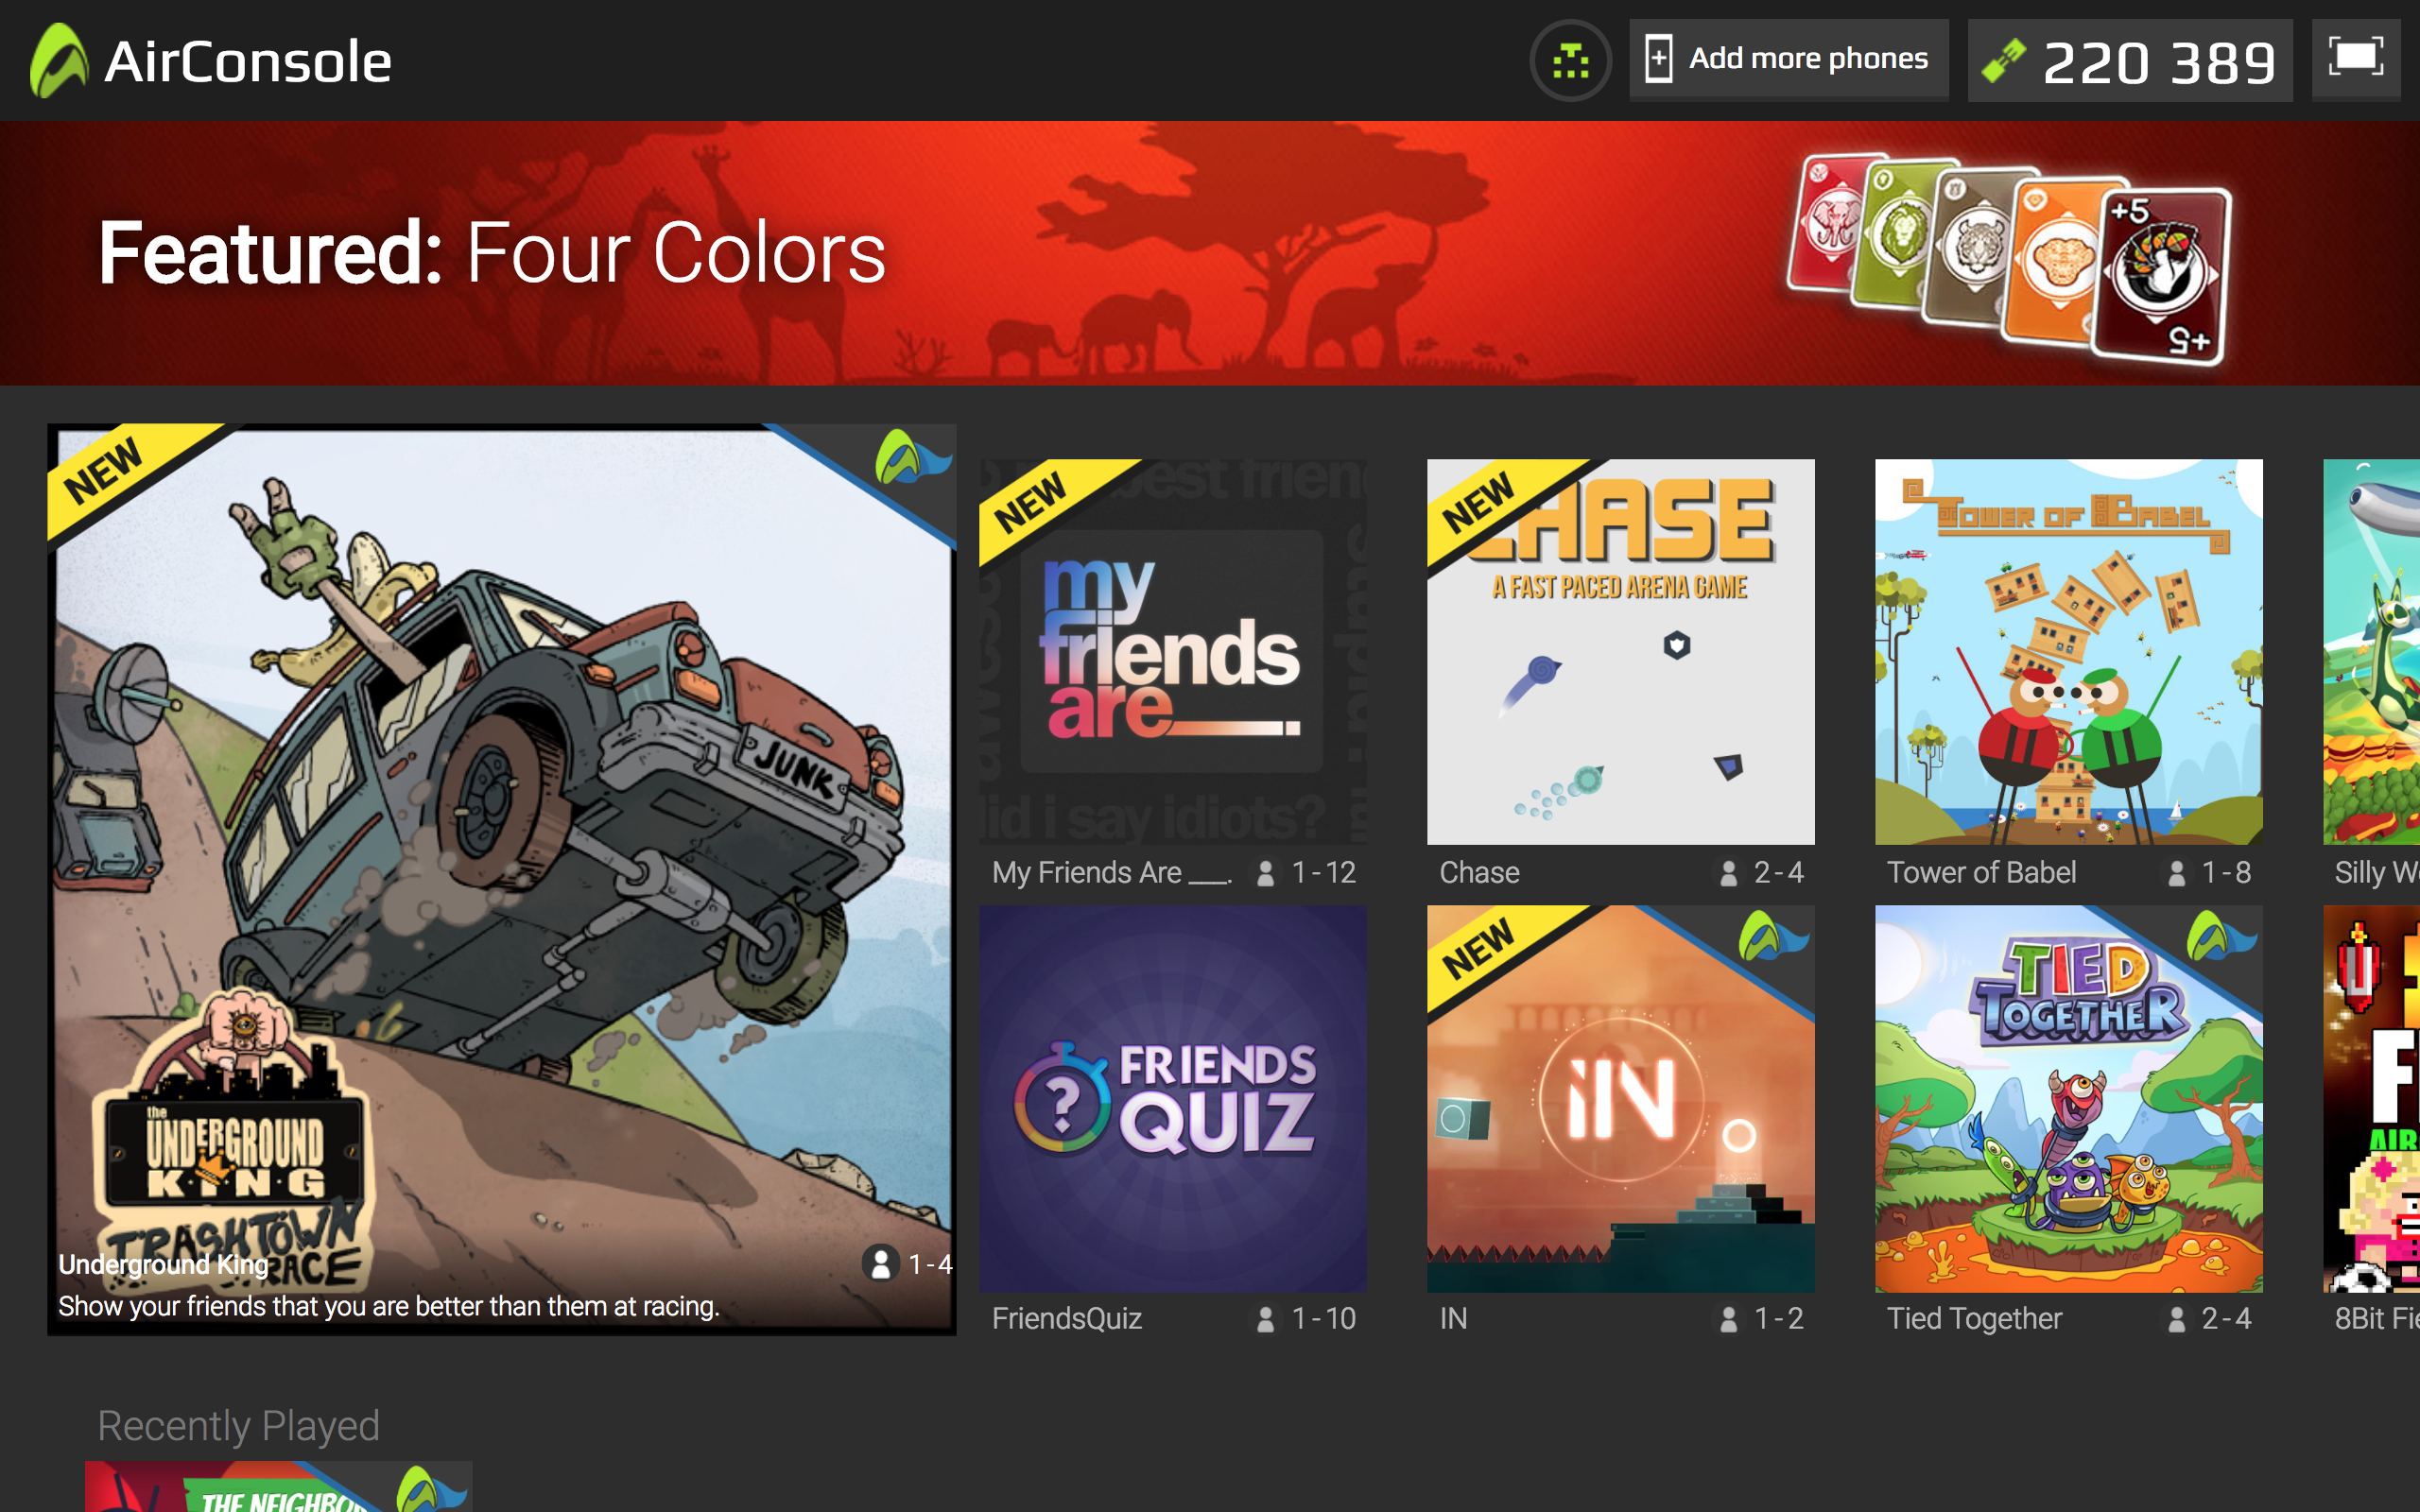
\includegraphics[scale=0.3]{Gambar/con3_play1}
	\caption{Halaman pada \textit{PC} yang menunjukan berbagai permainan yang dapat dipilih.}
	\label{fig:21_con3_play1}
\end{figure}

\begin{figure}[H]
	\centering
	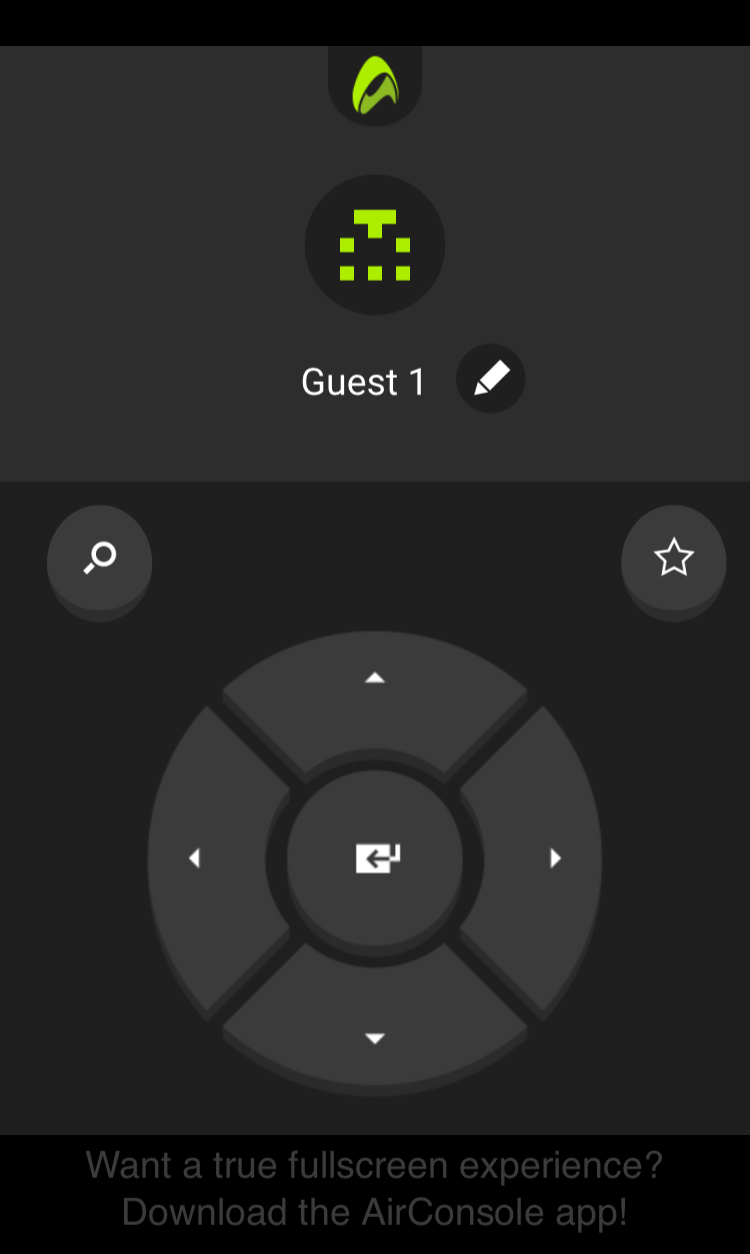
\includegraphics[scale=0.3]{Gambar/air4_play1}
	\caption{Halaman pada \textit{smartphone} yang berfungsi sebagai pengendali.}
	\label{fig:22_air4_play1}
\end{figure}

Dalam analisis ini, penulis memilih untuk memainkan permainan yang bernama The Neighborhood. Permainan ini sejenis permainan Angry Birds. Permainan ini bercerita tentang dua kelompok yang bertetangga, dimana kelompok tersebut bermusuhan dan berusaha untuk saling menghancurkan satu sama lain. Tujuan dari permainan ini yaitu lebih dulu menghancurkan anggota kelompok tetangga. Setelah memilih permainan tersebut, halaman pada \textit{PC} dan \textit{smartphone} akan berubah. Pada \textit{smartphone}, pemain akan diminta untuk merubah mode tampilan \textit{smartphone} menjadi \textit{landscape}.

\begin{figure}[H]
	\centering
	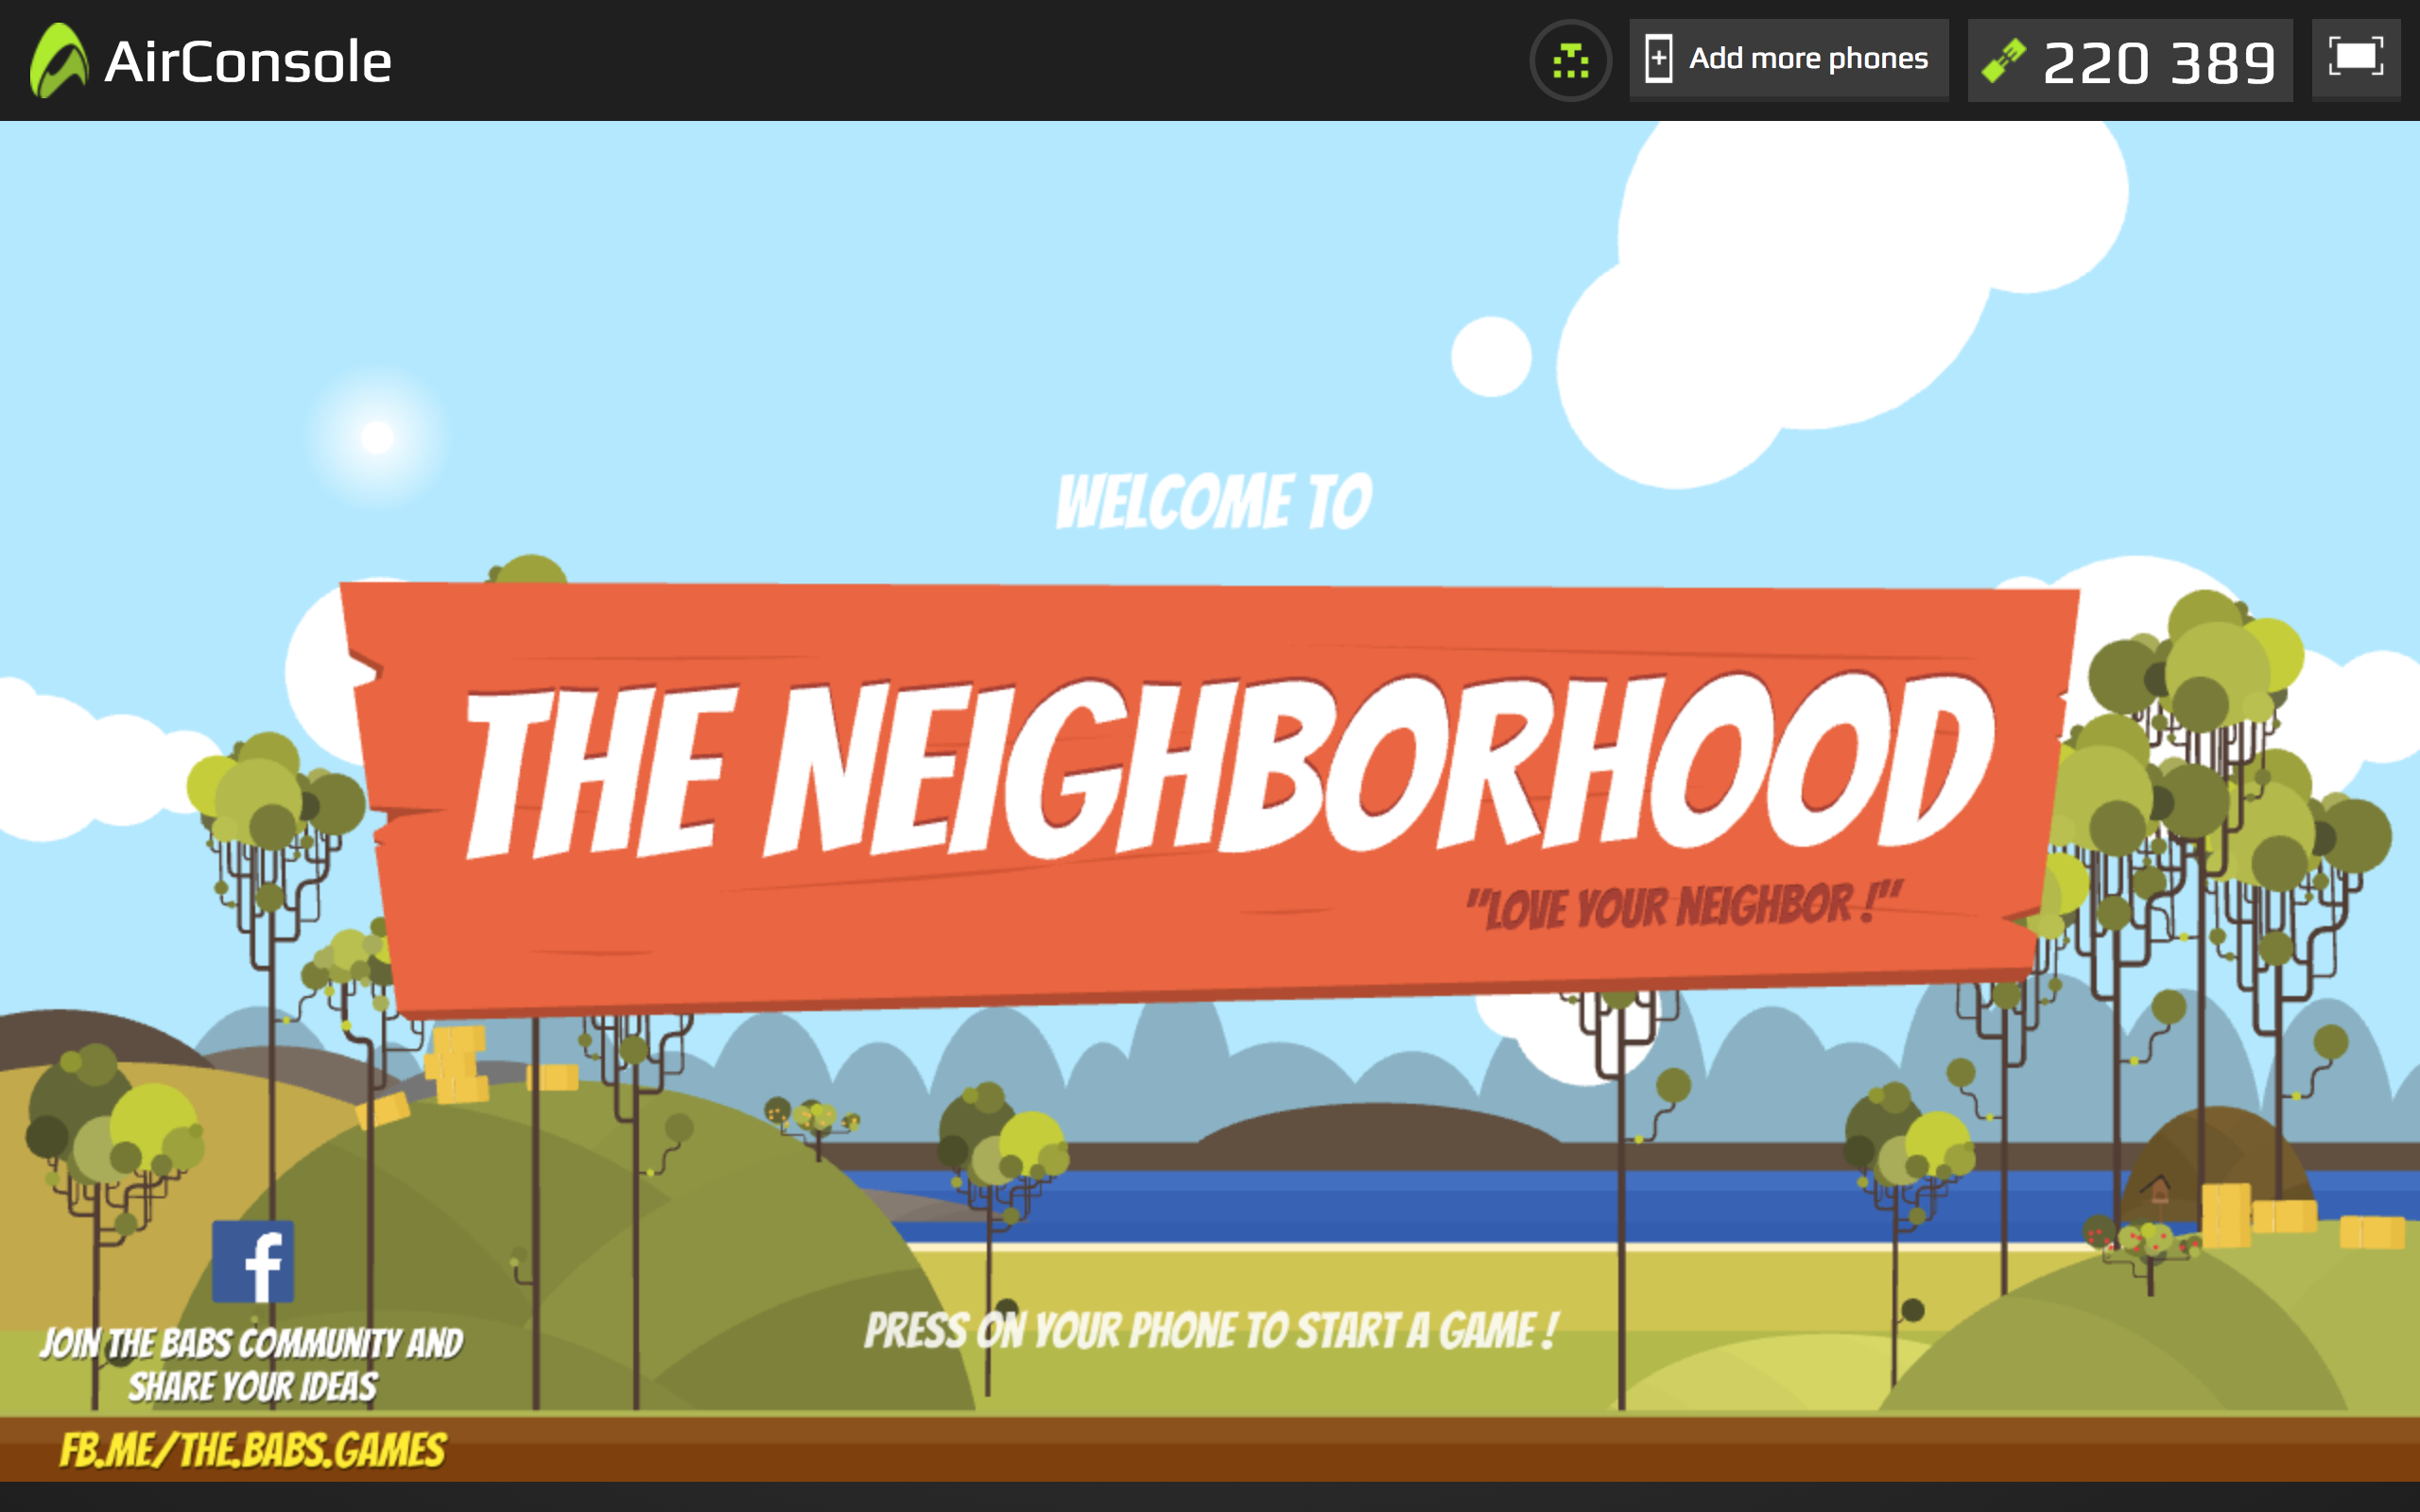
\includegraphics[scale=0.3]{Gambar/con5_play3}
	\caption{Halaman awal permainan The Neighborhood pada \textit{PC}.}
	\label{fig:23_con5_play3}
\end{figure}

\begin{figure}[H]
	\centering
	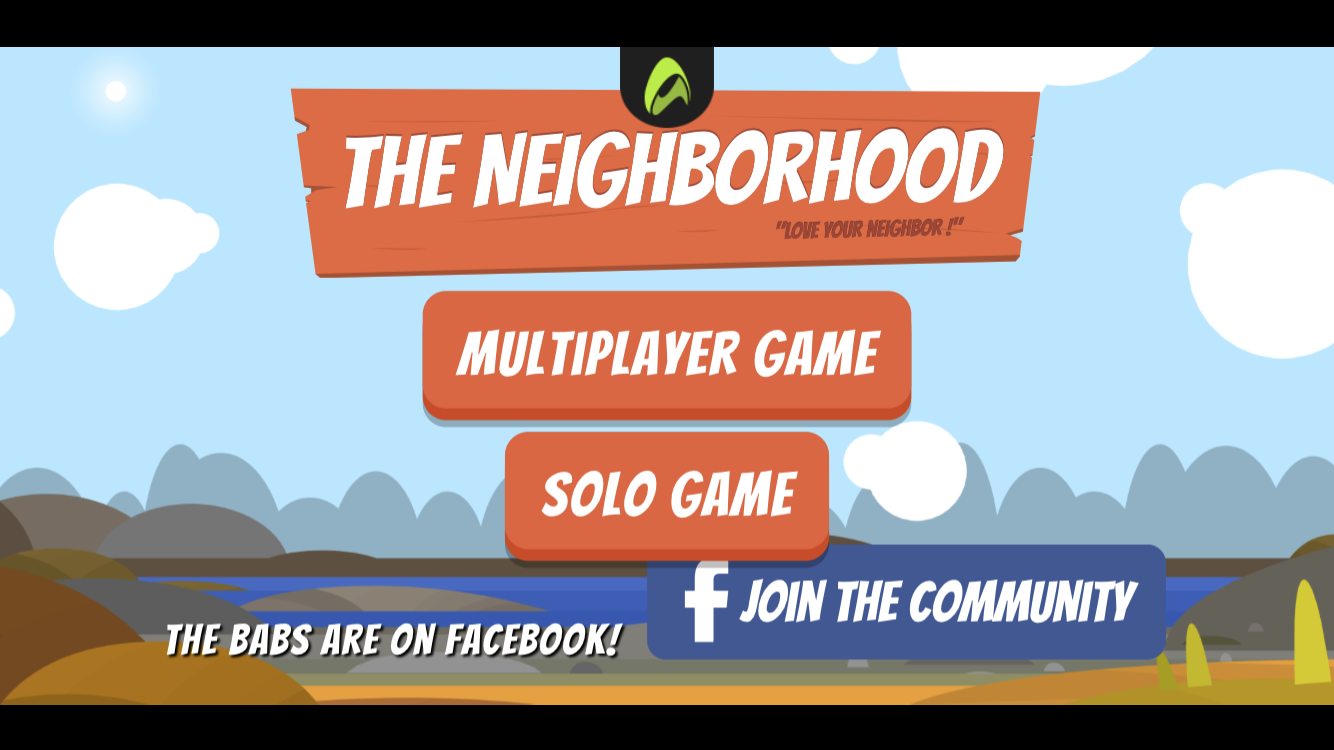
\includegraphics[scale=0.3]{Gambar/air6_play3}
	\caption{Halaman awal permainan The Neighborhood pada \textit{smartphone}.}
	\label{fig:24_air6_play3}
\end{figure}

Cara bermain dari permainan tersebut yaitu dengan menggunakan \textit{smartphone}, dimana pemain harus menekan layar \textit{smartphone}, kemudian menariknya sesuai dengan arah yang berlawanan dengan lawan, lalu melepas jari dari layar \textit{smartphone} dengan tujuan untuk melempar suatu benda dari ketapel. Semakin jauh pemain menarik, maka lontaran benda tersebut akan semakin kencang mengenai lawan.

\begin{figure}[H]
	\centering
	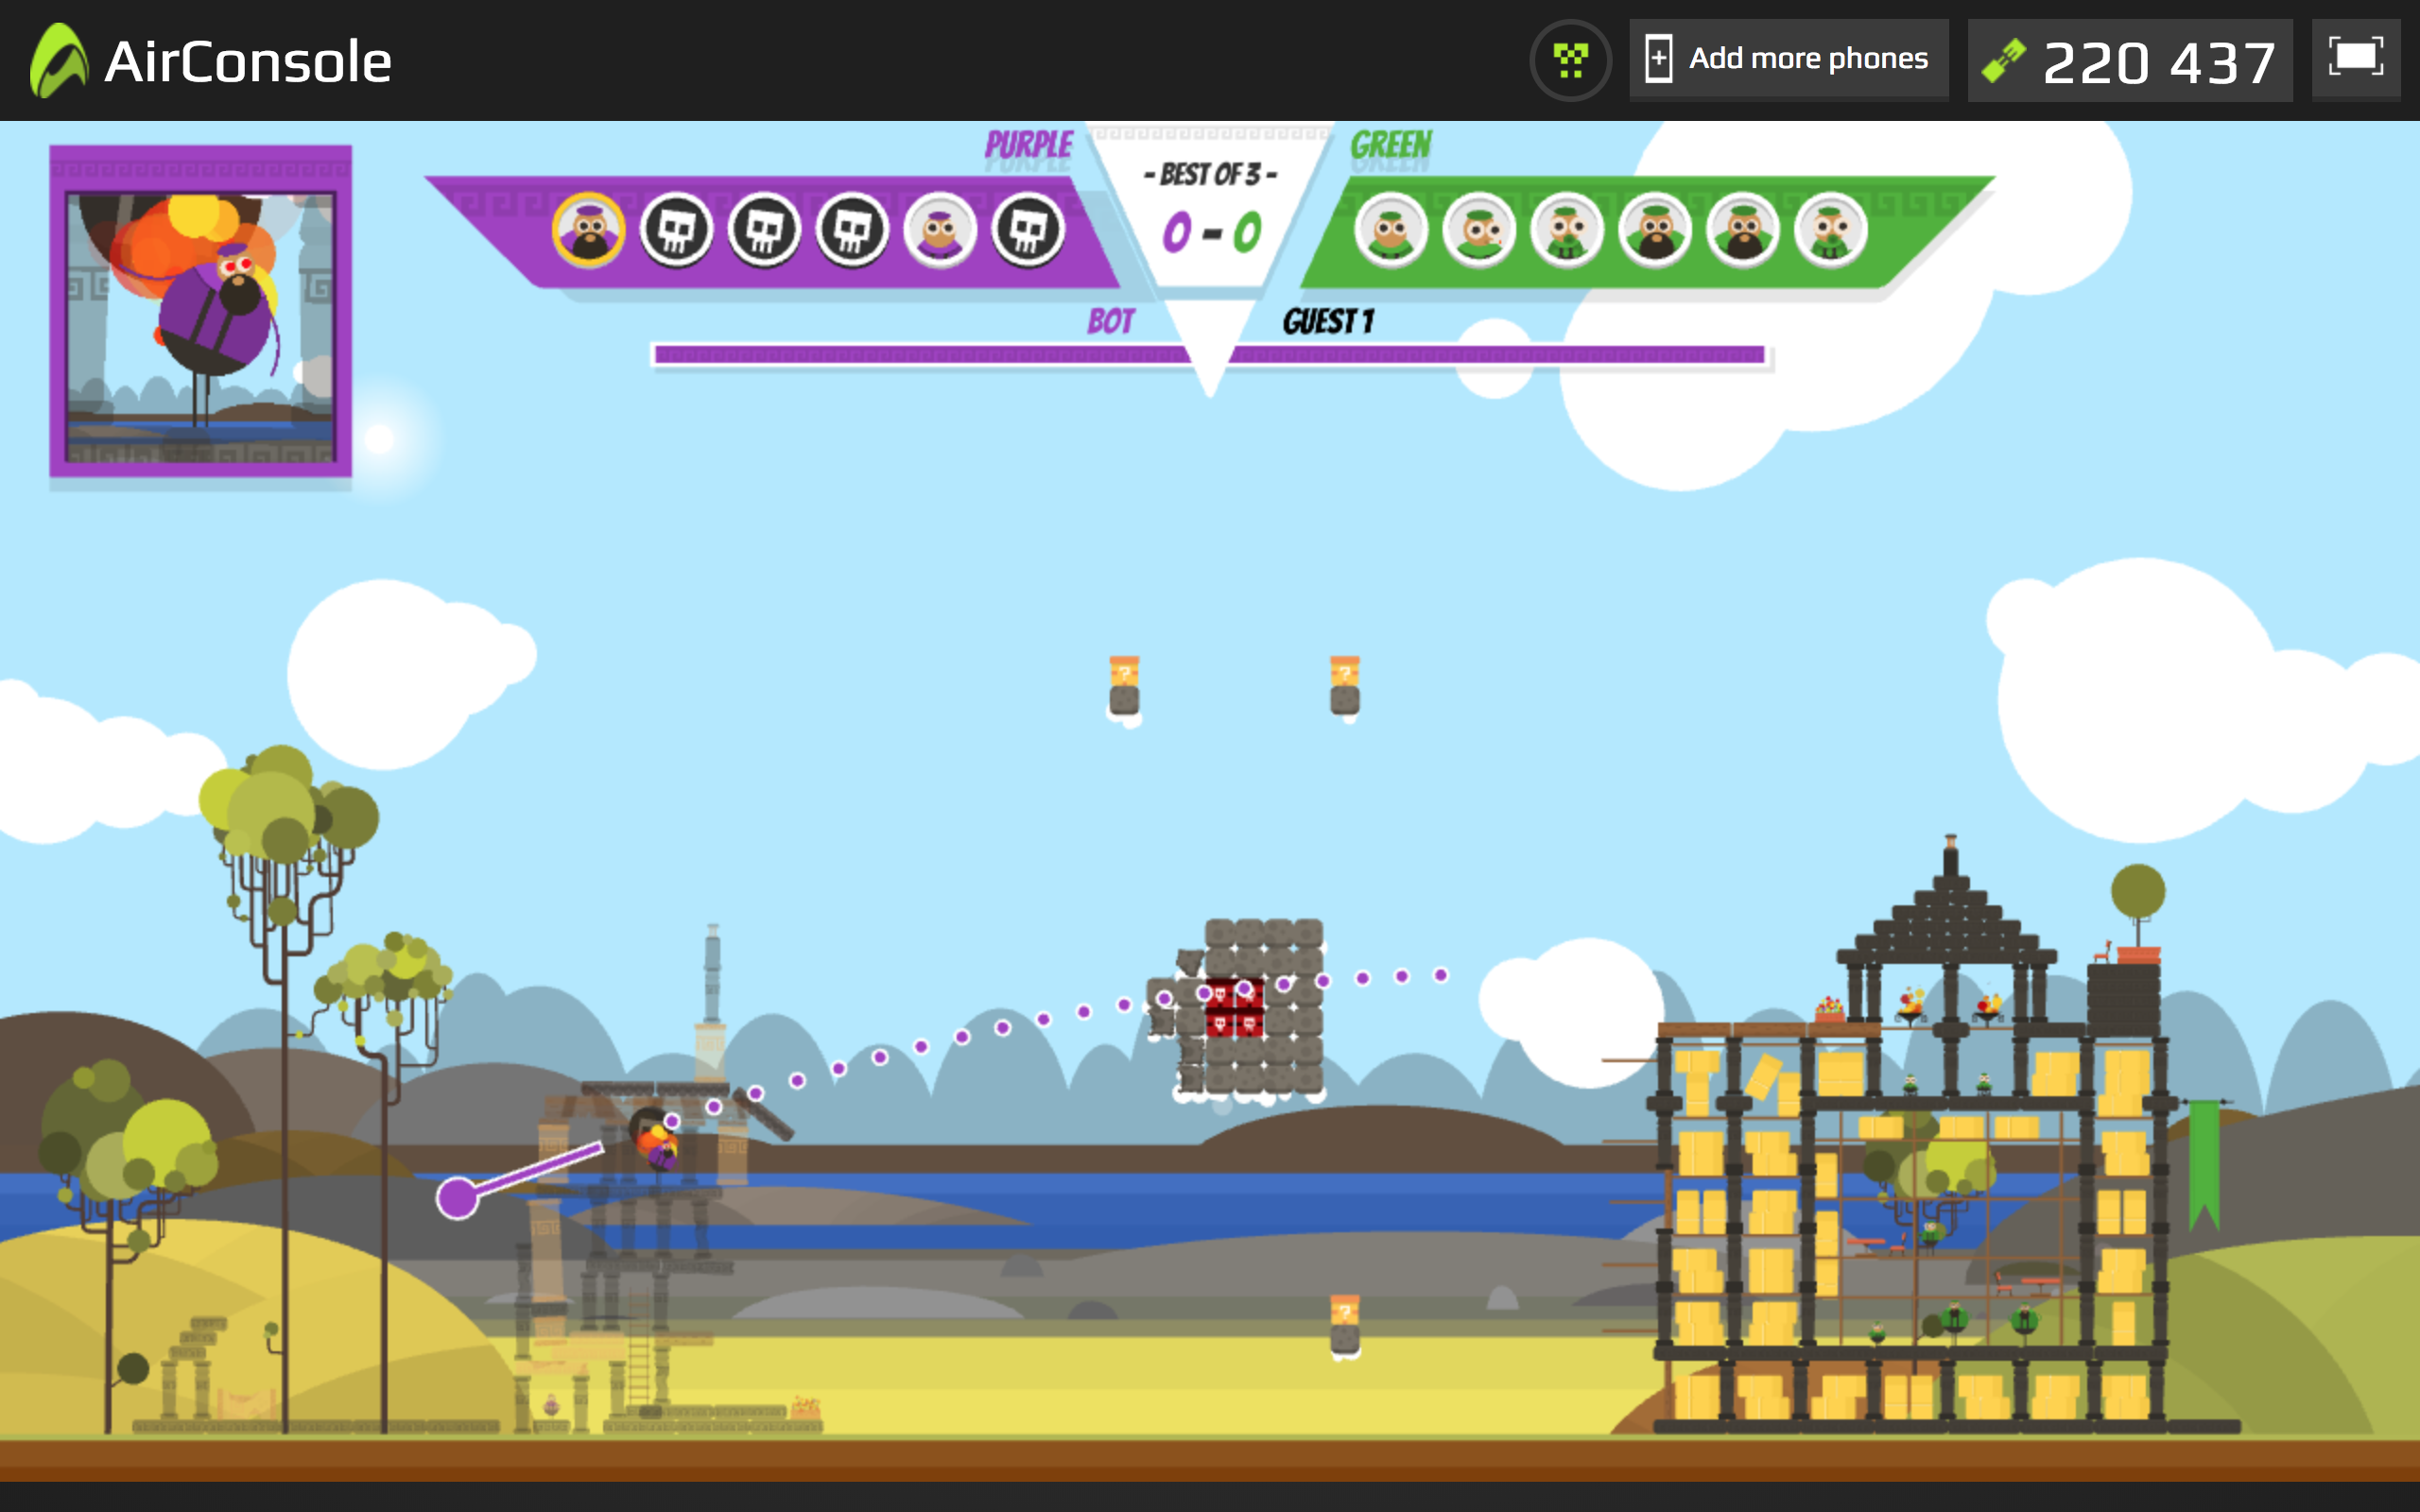
\includegraphics[scale=0.3]{Gambar/con7_play5}
	\caption{Halaman pada \textit{PC} dimana permainan sedang berlangsung.}
	\label{fig:25_con7_play5}
\end{figure}

\begin{figure}[H]
	\centering
	
\includegraphics[scale=0.3]{Gambar/air7_play4}
	\caption{Halaman pada \textit{smartphone} dimana permainan sedang berlangsung.}
	\label{fig:26_air7_play4}
\end{figure}

Apabila memenangkan permainan tersebut, maka pemain dapat memilih untuk keluar dari permainan atau melanjutkan permainannya kembali.

\begin{figure}[H]
	\centering
	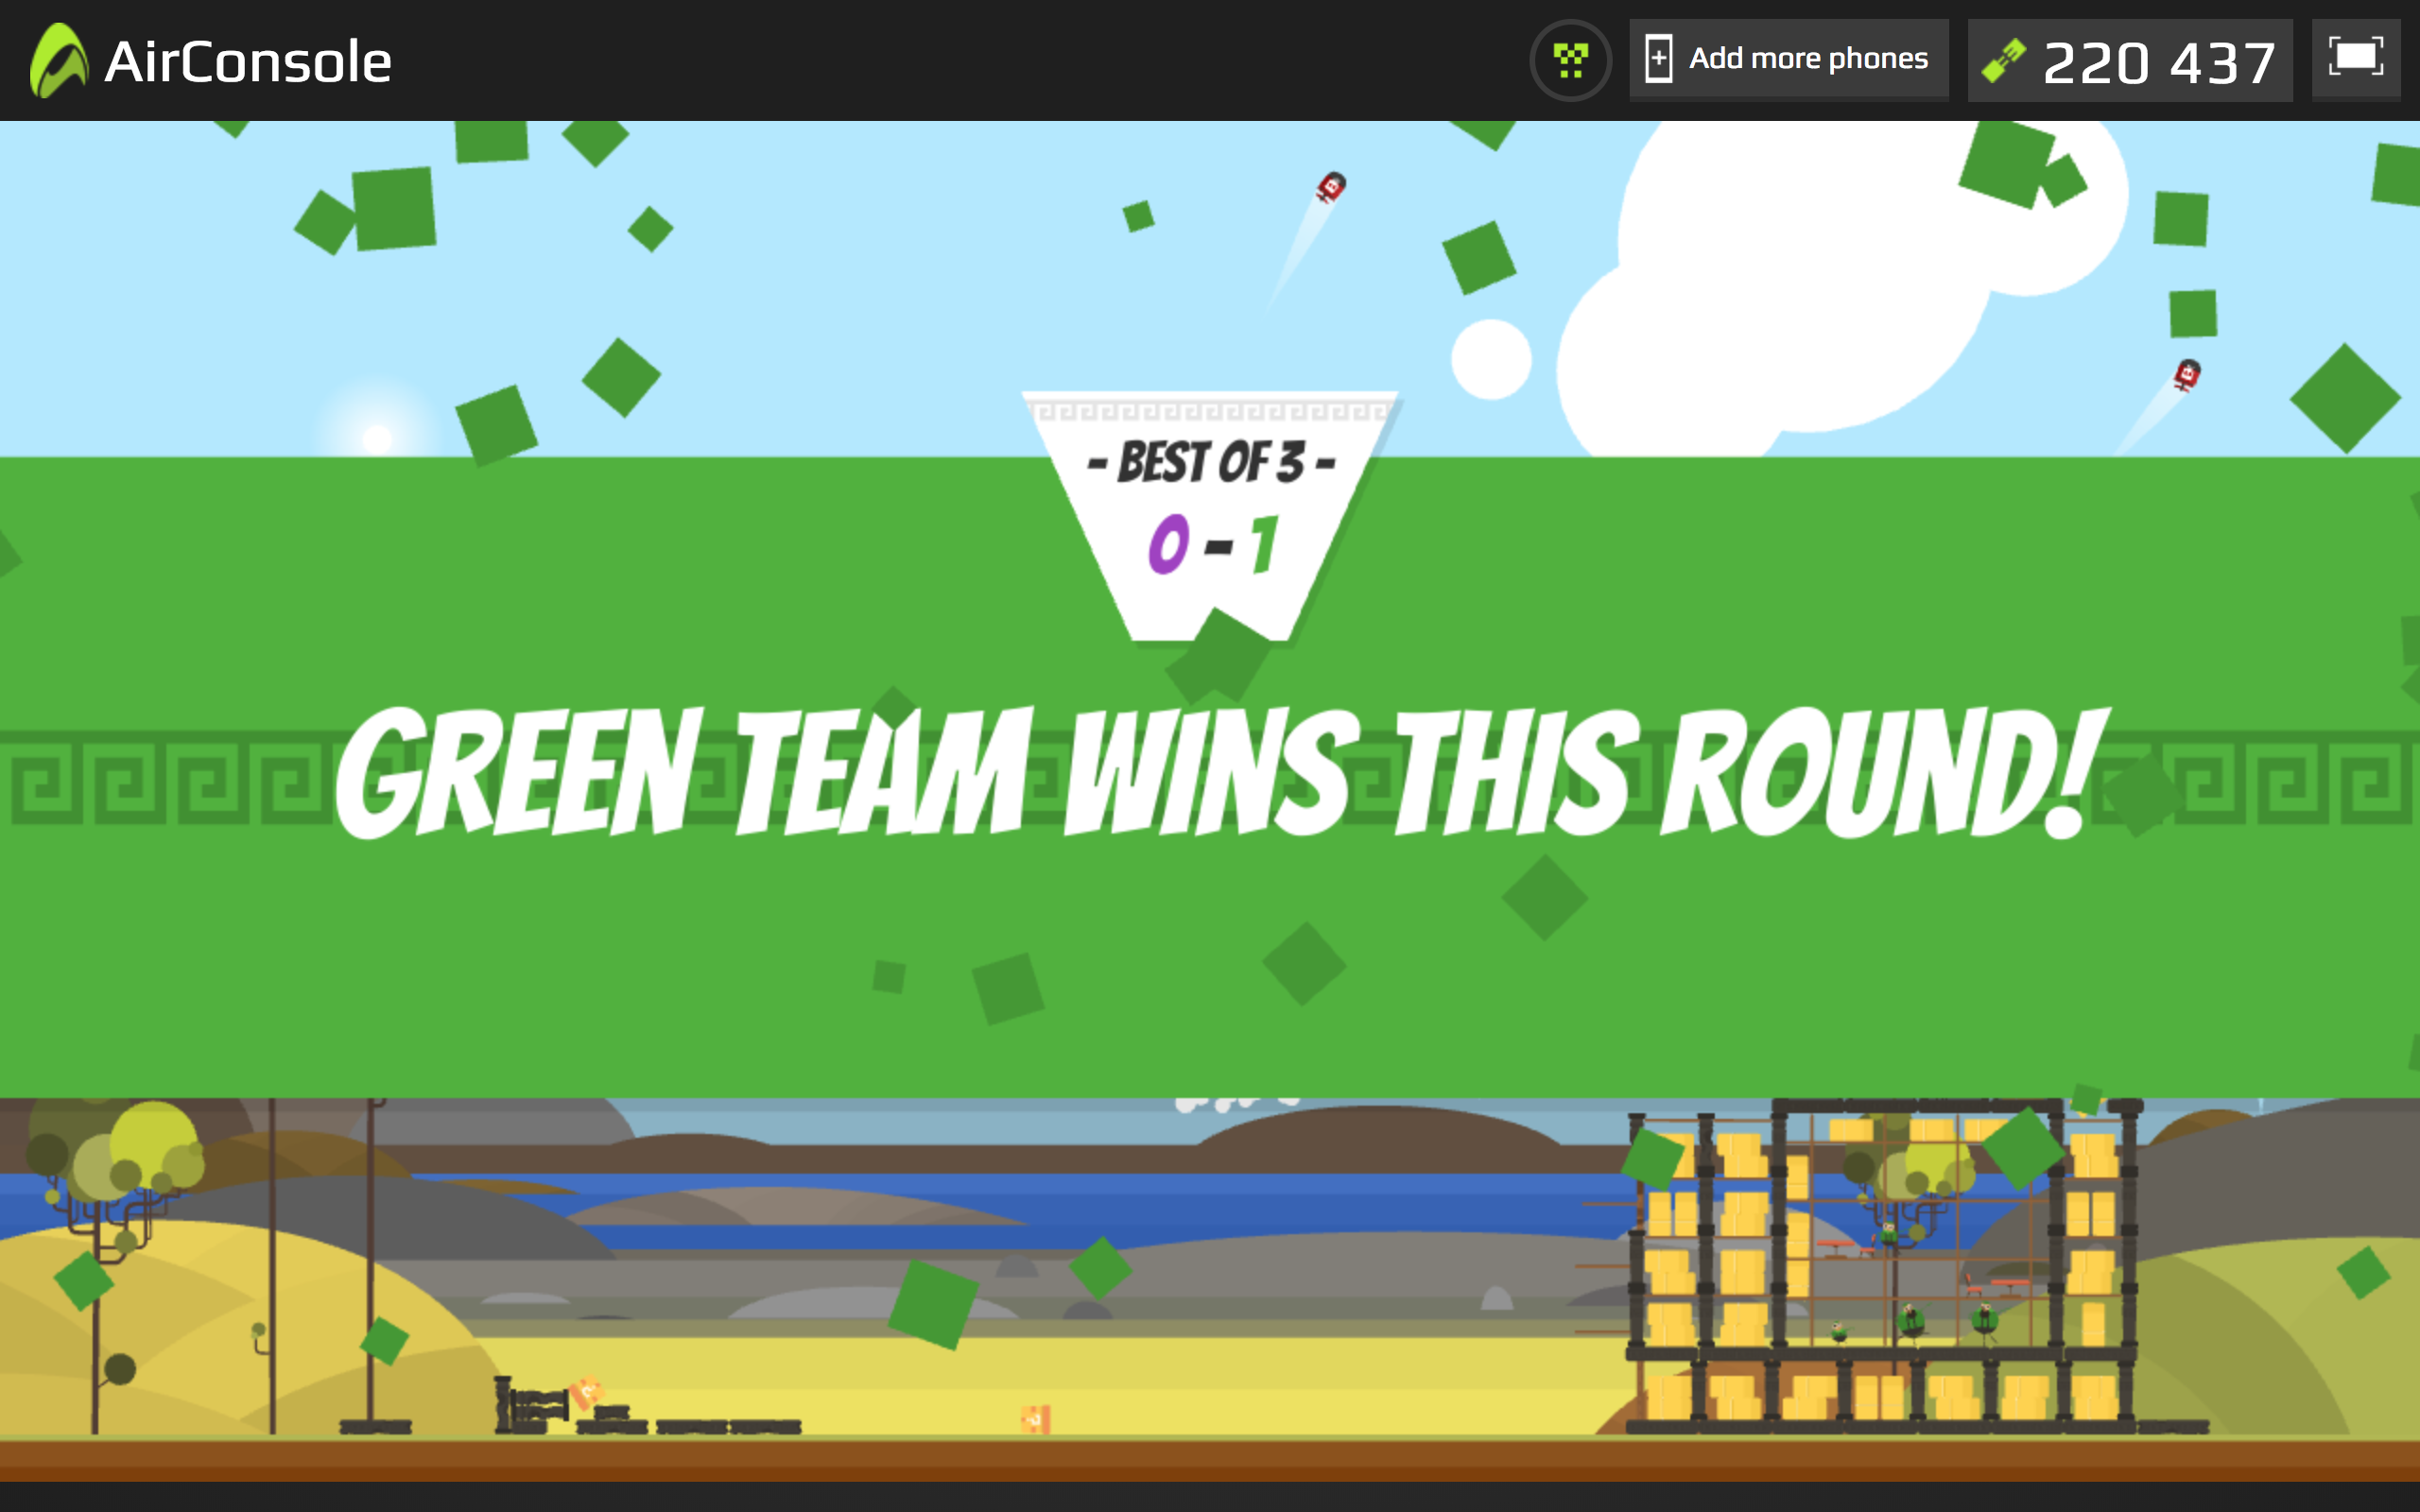
\includegraphics[scale=0.3]{Gambar/con8_play6}
	\caption{Halaman pada \textit{PC} apabila permainan sudah dimenangkan.}
	\label{fig:27_con8_play6}
\end{figure}

\begin{figure}[H]
	\centering
	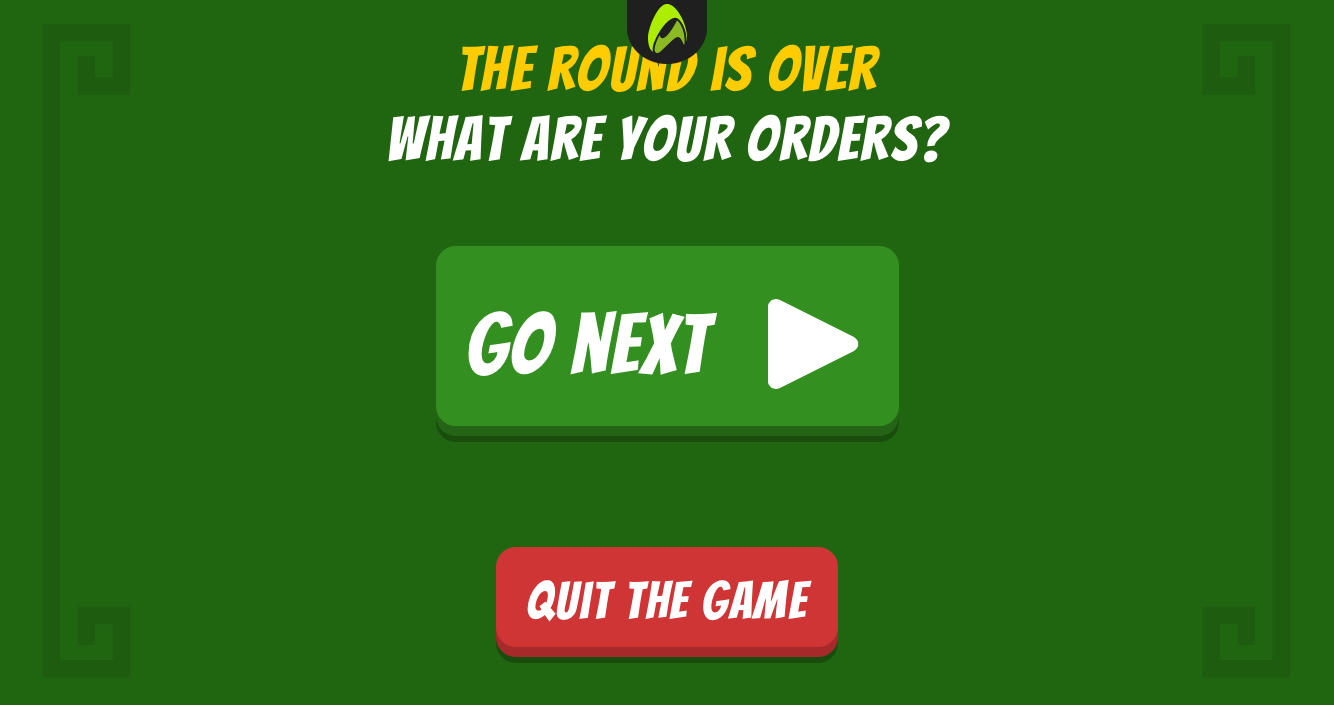
\includegraphics[scale=0.3]{Gambar/air8_finish}
	\caption{Halaman pada \textit{smartphone} apabila permainan sudah dimenangkan.}
	\label{fig:28_air8_finish}
\end{figure}

Dari ketiga percobaan yang sudah dilakukan, ada beberapa hal yang dapat diperbaiki dari permainan berbasis web tersebut. Percobaan pertama menunjukan hasil yang bagus, dimana koneksi antara \textit{smartphone} dan \textit{PC} tidak putus saat permainan berlangsung, dan juga tidak ada keterlambatan antara gerakan pada \textit{smartphone} dan \textit{PC}. Pada percobaan kedua, apabila \textit{browser} pada \textit{PC} ditutup pada saat permainan berlangsung, maka koneksi akan terputus. Tetapi, tampilan pada \textit{smartphone} tidak menunjukan bahwa adanya koneksi yang terputus, sehingga pemain tidak mengetahui apakah permainan masih dapat berlangsung atau tidak. Tampilan hanya akan langsung kembali pada halaman awal permainan. Begitupun dengan percobaan ketiga, apabila \textit{browser} pada \textit{smartphone} ditutup pada saat permainan sedang berlangsung, maka koneksi akan terputus. Tampilan pada \textit{PC} hanya menunjukan tanda kecil bahwa telah terjadi pemutusan koneksi pada \textit{smartphone}, yaitu tanda x pada bagian atas tampilan yang ditunjukan seperti gambar berikut:

\begin{figure}[H]
	\centering
	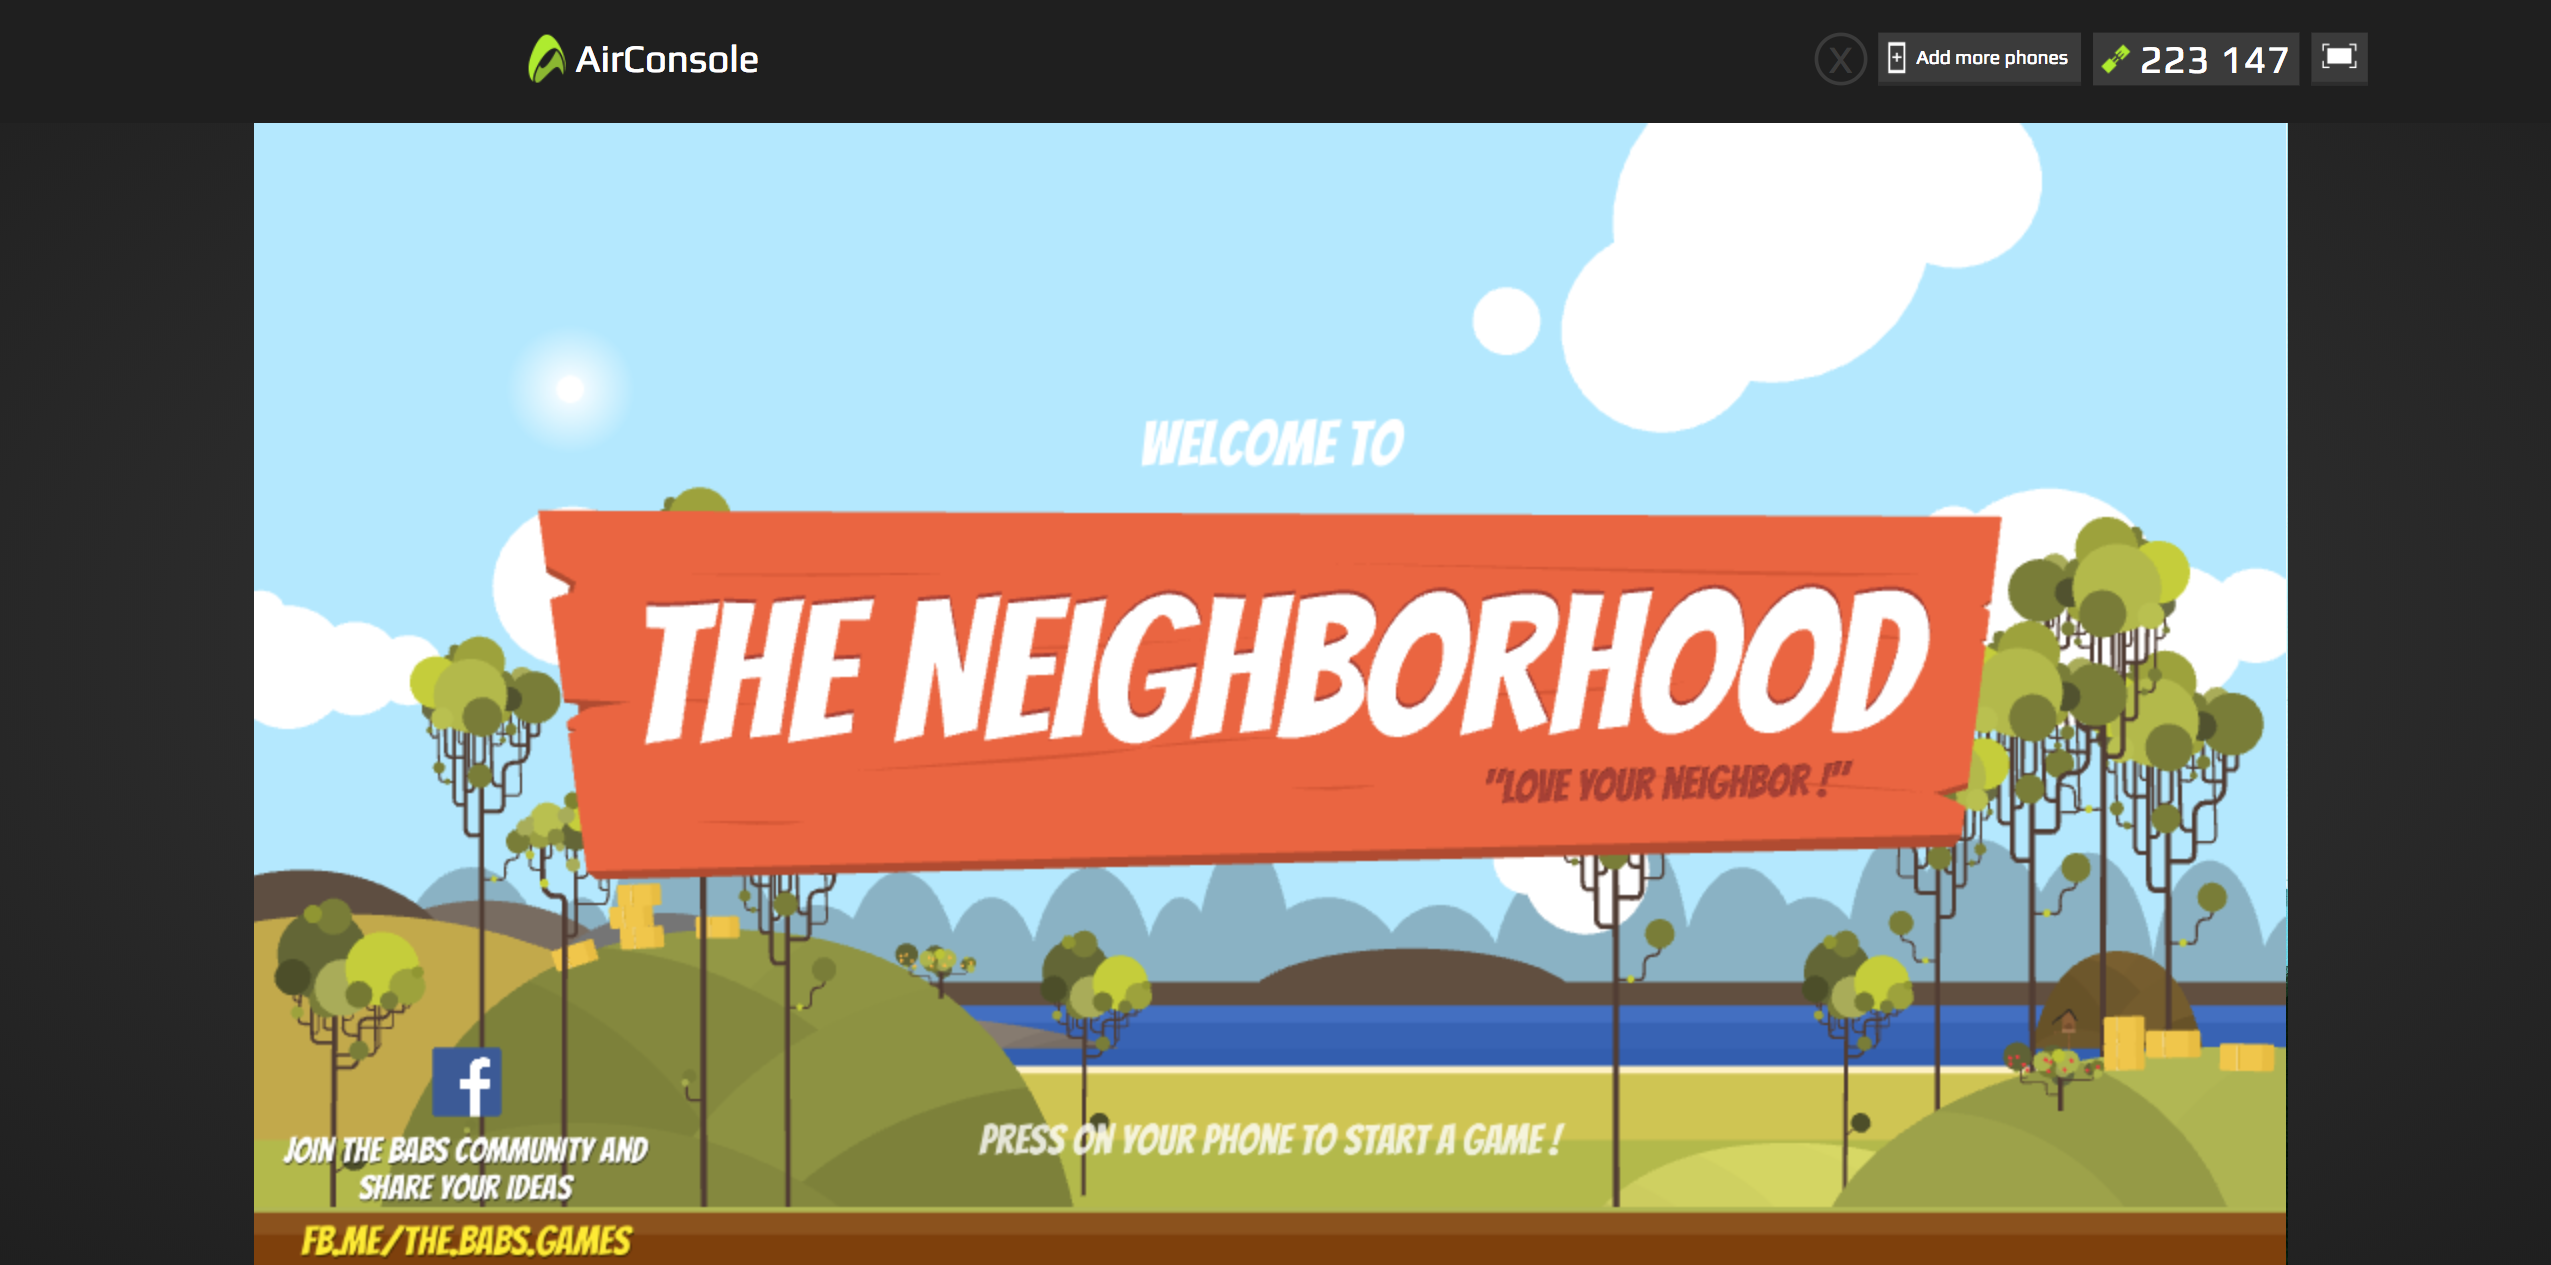
\includegraphics[scale=0.3]{Gambar/con9_play7}
	\caption{Halaman pada \textit{PC} yang menunjukan pemutusan koneksi.}
	\label{fig:29_con9_play7}
\end{figure}

Perbaikan yang dapat dilakukan adalah dengan memberi \textit{feedback} yang lebih jelas pada pemain, apabila ada kesalahan pada aplikasi yang terjadi seperti pemutusan koneksi. Dengan begitu, pemain akan lebih mengetahui bahwa koneksi dapat saja terputus dan tidak dapat melanjutkan permainannya.

\section{Analisis Sequence Diagram}
\label{sequence}

Pada analisis ini dilakukan pengamatan pada jalannya koneksi \textit{socket.io} antara \textit{server} dan \textit{client}. Hal-hal yang dianalisis adalah bagaimana koneksi tersambung di awal permainan, bagaimana data-data yang dibutuhkan dikirim melalui koneksi tersebut, hingga koneksi antara \textit{client} dan \textit{server} terputus. Analisis dilakukan dengan menggunakan \textit{developer tools} yang tersedia pada \textit{web browser} untuk mengamati koneksi \textit{client}, dan \textit{terminal} untuk mengamati koneksi \textit{server}.

\subsection{Sequence Diagram JoinRoom}

%Sediain gambar server dan client saat si host berhasil konek ke socket.io


Pada awal permainan, \textit{client} pertama yang melakukan koneksi pada \textit{server} adalah \textit{desktop computer}, yang berperan sebagai \textit{host} dalam permainan.\textit{Host} akan menyediakan suatu kode yang berguna sebagai \textit{room} untuk kedua pemain yang akan bergabung dengan melakukan koneksi ke \textit{server}. \textit{Room} yang disediakan hanya akan menerima tiga \textit{client} saja, yaitu \textit{host}, \textit{player1}, dan \textit{player2}. 

Setelah berhasi melakukan koneksi, maka \textit{client} akan memiliki \textit{socket.id} yang berfungsi sebagai tanda pengenal unik, dan kode \textit{room} dimana proses pengiriman dan penerimaan data hanya dapat dilakukan didalam \textit{room} tersebut. 

Setelah \textit{client} pertama berhasil tersambung, selanjutnya para pemain yang akan bergabung akan melakukan koneksi pada \textit{server}. Pemain akan menggunakan \textit{smartphone} yang akan berfungsi sebagai \textit{controller} permainan. Untuk melakukan koneksi, pemain harus memasukan kode \textit{room} yang telah disediakan \textit{host} agar dapat bergabung. Pada proses ini, akan dilakukan pengecekan oleh \textit{server}, apakah kode \textit{room} yang telah dikirim oleh \textit{client} tersedia atau tidak. Apabila \textit{room} tersedia, maka pemain akan berhasil bergabung, dan apabila tidak tersedia, maka pemain tidak dapat bergabung.

Pengecekan tambahan yang dilakukan pada proses ini adalah jumlah \textit{client} yang sudah ada didalam \textit{room}. Apabila jumlahnya masih kurang dari tiga, maka \textit{room} masih membuka koneksi bagi yang akan bergabung. Apabila \textit{room} sudah diisi oleh tiga \textit{client}, maka \textit{room} tidak akan menerima \textit{client} yang akan bergabung lagi.

%sediain gambar client dan sever saat si pemain request connection 

Pada tahap ini, halaman pada \textit{client} dan \textit{server} akan menuju ke halaman pemilihan karakter. Pada jalannya permainan, \textit{socket.id} yang dimiliki oleh masing-masing \textit{client} akan berperan sangat penting untuk proses pengiriman data. Pada koneksi \textit{socket.io}, apabila suatu \textit{client} berpindah halaman dari satu \textit{file} \textit{html} menuju \textit{file} \textit{html} lainnya, koneksi tersebut akan terputus dan akan melakukan koneksi ulang kembali. Dengan begitu, \textit{socket.id} yang dimiliki oleh \textit{client} pun akan berganti karena proses perpindahan \textit{file} \textit{html} dan koneksi ulang. 

Agar koneksi yang dimiliki \textit{client} tidak terputus dan \textit{socket.id} yang dimiliki tidak berganti, maka untuk proses perpindahan halaman harus dibutuhkan satu \textit{file} \textit{html} saja. Hal tersebut dapat dilakukan dengan cara menggunakan \textit{syntax} yang disediakan oleh \textit{html}, yaitu \textit{template}. 

%sediain gambar screenshot syntax template html untuk macem2 halaman

Dengan menggunakan \textit{template} pada satu \textit{file} \textit{html}, maka proses perpidahan halaman hanya akan terjadi didalam satu \textit{file} saja. Halaman yang akan ditunjukan kepada \textit{client} akan dilakukan dengan cara berpindah dari satu \textit{template} ke \textit{template} yang lainnya. Dengan begitu, koneksi \textit{socket.io} tidak akan terputus, dan \textit{socket.id} milik \textit{client} tidak akan berganti.

Setelah masuk ke halaman pemilihan karakter, pemain dapat memilih karakter yang akan dimainkan. Pada \textit{smartphone}, akan ditampilkan daftar karakter yang dapat dipilih, dan pada \textit{desktop}, akan ditampilkan karakter mana yang telah dipilih oleh para pemain untuk dimainkan.

%sediain gambar smartphone yang isinya daftar pemain, sama desktop yang nunjukin karakter mana yang dipilih.

Agar karakter yang dipilih pada \textit{smartphone} sesuai dengan yang ditunjukan oleh \textit{desktop}, maka dibutuhkan proses pengiriman data didalam koneksi \textit{socket.io}. Saat pemain memilih karakter, pemain akan mengirimkan suatu \textit{event} kepada \textit{server} dengan parameter yang berisi \textit{socket.id} dan \textit{value} yang menandakan karakter mana yang dipilih. Setelah \textit{event} tersebut sampai pada \textit{server}, akan dilanjutkan kembali kepada \textit{client} yang berperan sebagai \textit{host}. Pada tahap ini, \textit{host} akan menerima \textit{event} tersebut dan memprosesnya. Parameter \textit{value} yang dikirimkan oleh pemain dibutuhkan oleh \textit{host} untuk menampilkan karakter yang dipilih, sedangkan \textit{socket.id} berfungsi untuk mengetahui pemain mana yang memilih karakter tertentu sehingga dapat menampilkannya dengan tepat.

%sediain gambar screenshot code event charSelecting, terus tampilin juga dev tools sama terminal

Setelah karakter ditampilkan pada \textit{desktop}, maka pemain dapat menekan tombol \textit{choose} yang berarti pemain sudah memutuskan untuk memakai karakter tersebut di permainan. Pada proses ini, akan dilakukan pengecekan pada \textit{server}, apakah kedua pemain sudah menetapkan karakter yang akan dimainkan. Apabila belum ada atau hanya satu pemain yang sudah menetapkan karakter, maka permainan belum bisa dimulai. Permainan akan dimulai apabila kedua pemain telah menetapkan karakter, yang kemudian halaman akan berpindah pada halaman permainan.

%sediain gambar pengecekan udah ada pemain yang milih atau belum.

Kedua pemain yang telah menetapkan karakter akan ditampilkan halaman permainan, begitu juga dengan \textit{host}. Pada halaman \textit{desktop}, pertama-tama akan ditampilkan \textit{countdown} selama tiga detik sebelum para pemain dapat menggunakan \textit{smartphone}nya sebagai \textit{controller}. Apabila \textit{countdown} sudah habis, maka permainan dapat dimulai.

Pemain akan menekan tombol yang ditampilkan di \textit{smartphone} secara terus menerus. Pada tahap ini, apabila tombol ditekan, pemain akan mengirimkan suatu \textit{event} pada \textit{server} dengan parameter berisi \textit{socket.id}. Setelah \textit{event} tersebut sampai ke \textit{server}, maka akan dilanjutkan kembali menuju \textit{client} yang berperan sebagai \textit{host}. \textit{Host} akan memproses \textit{event} tersebut, dan menyesuaikan pemain mana yang memiliki \textit{id} sesuai dengan yang diterima. Karakter akan mulai bergerak sesuai dengan \textit{id} para pemain. Agar karakter yang dimainkan dapat mencapai garis akhir, maka pemain harus menekan tombol pada \textit{smartphone} terus menerus.

%sediain gambar screenshot si player yang neken tombol, terus tampilin terminal yang nunjukin canvas api animation.

Apabila sudah ada pemain yang menyentuh garis akhir, maka permainan pun akan berakhir dan halaman akan berubah menuju ke halaman pemenang. Pada saat permainan berakhir, akan dikirimkan suatu \textit{event} ke \textit{server} yang berisi parameter \textit{socket.id} dan \textit{value} untuk menampilkan pemain mana yang menang dan karakter mana yang dimilikinya. \textit{Event} tersebut kemudian dilanjutkan kembali ke \textit{host} lalu pemenang pun dapat ditampilkan. Pada tahap ini, pemain dapat memilih untuk keluar dari permainan dan kembali ke halaman utama.

%tampilin gambar winning page sama console dan si terminalnya juga


